\section{Results}
\label{sec:results}
\subsection{\psitwos-to-\jpsi ratio as functions of multiplicity}
With the signal yields determined from the fitting to dimuon invariant mass distributions, the efficiencies estimated from simulation and calibrated control sample, and the systematic uncertainties, the ratio of \psitwos and \jpsi production cross-sections are measured in each kinematic and multiplicity bin.
By integrating the double differential results over \pt($y$) one can obtain the ratio as functions of $y$(\pt).
And also the normalized ratio of total cross-sections as a function of normalized multiplicity can be obtained by integrating the double differential results over \pt and $y$ bins. The normalization of ratio is achieved simply by dividing the ratio in each multiplicity bin by the over-all ratio in integrated multiplicity region.
The normalized ratio of integrated production over \pt-$y$ as a function of PVNTRACKS is shown in Fig~\ref{Ratio}. We can see a decreasing trend for the ratio of prompt production with multiplicity getting larger. While for the ratio of production from $b$-hadron decay, no significantly decreasing trend is observed. 
\begin{figure}[!tbp]
    \begin{center}
      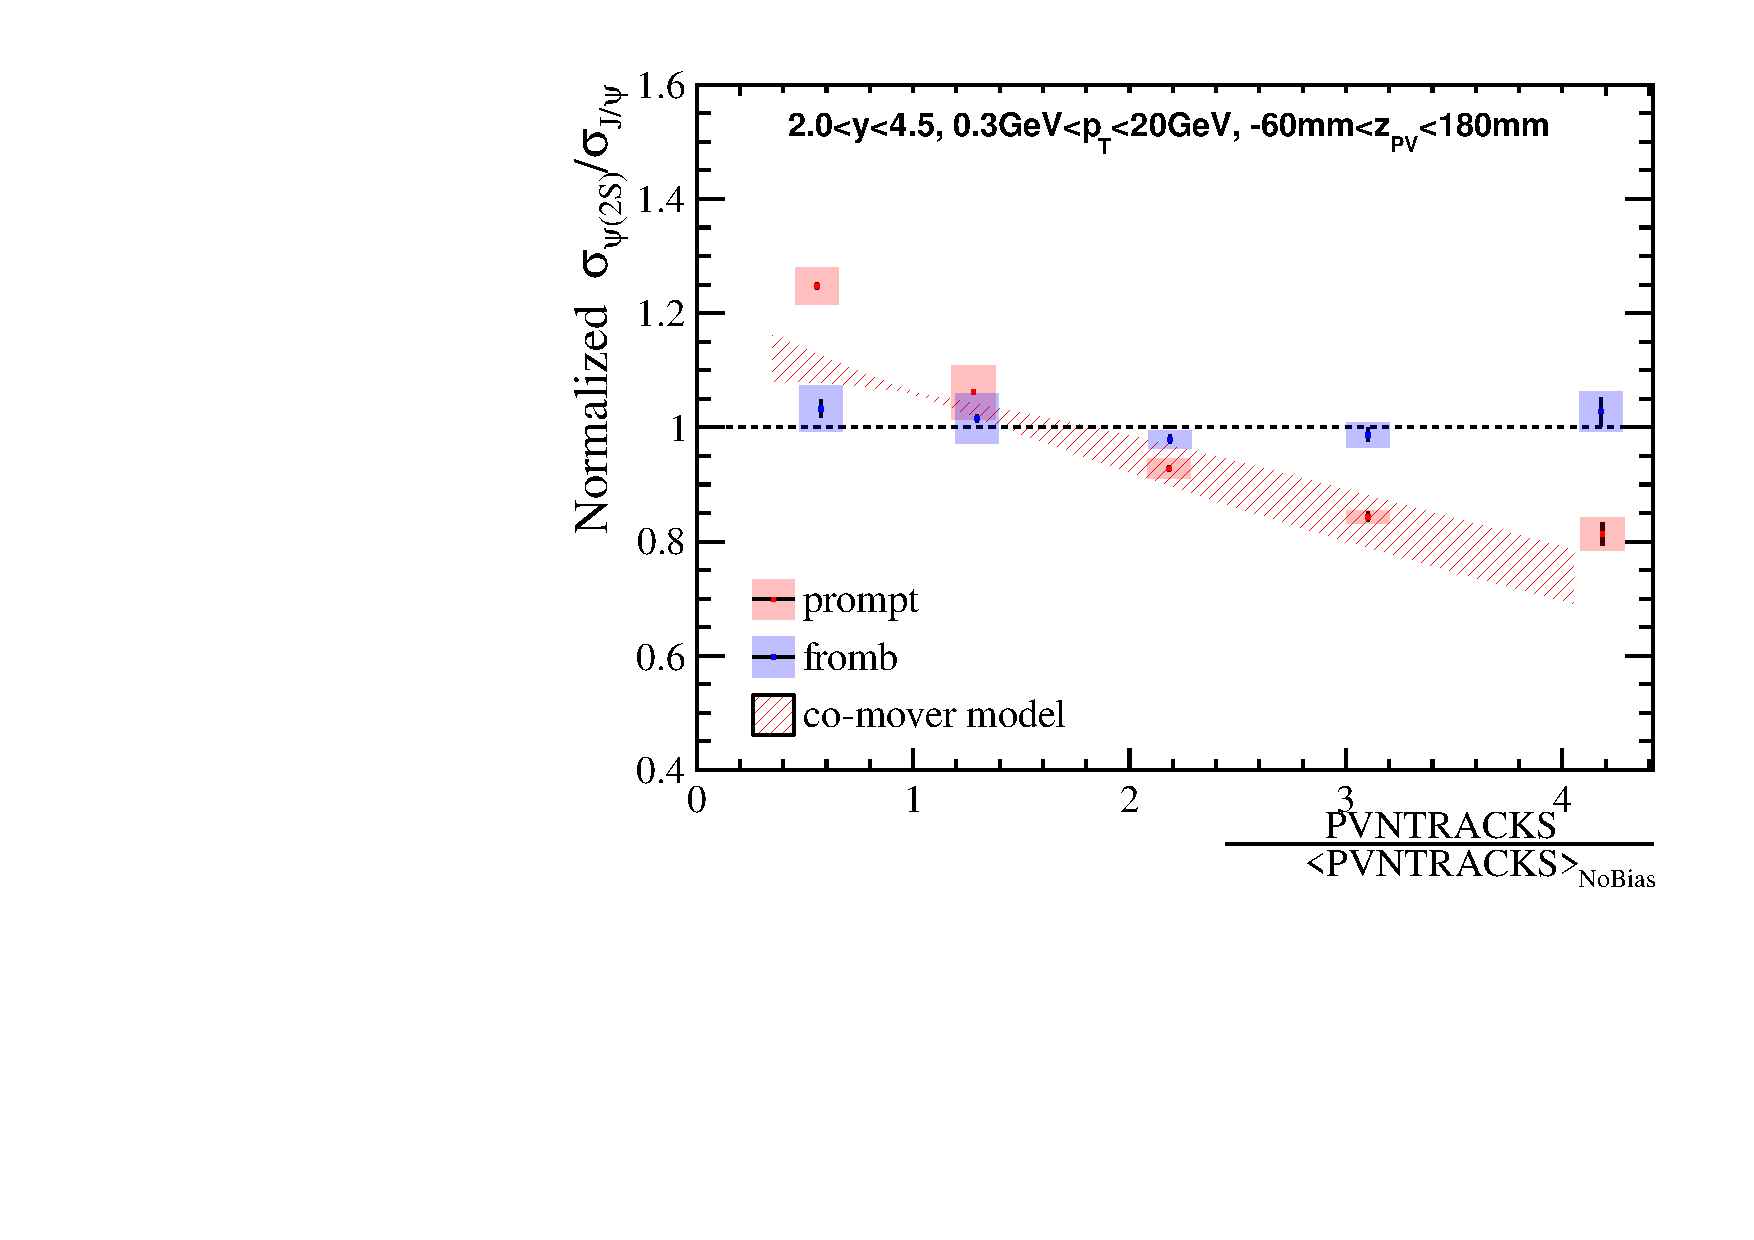
\includegraphics[width=0.8\linewidth]{pdf/Result/All.pdf}
    \end{center}
    \caption{ The ratio of integrated production over \pt-$y$ as a function of PVNTRACKS.
      }
    \label{Ratio}
\end{figure}
The ratio of production is also measured as a function of nBackTracks and nForwardTracks (see Figure ~\ref{RatioFB}), which are two mutual subsets of PVNTRACKS representing numbers of backward and forward tracks respectively. 
\begin{figure}[!tbp]
  \begin{center}
    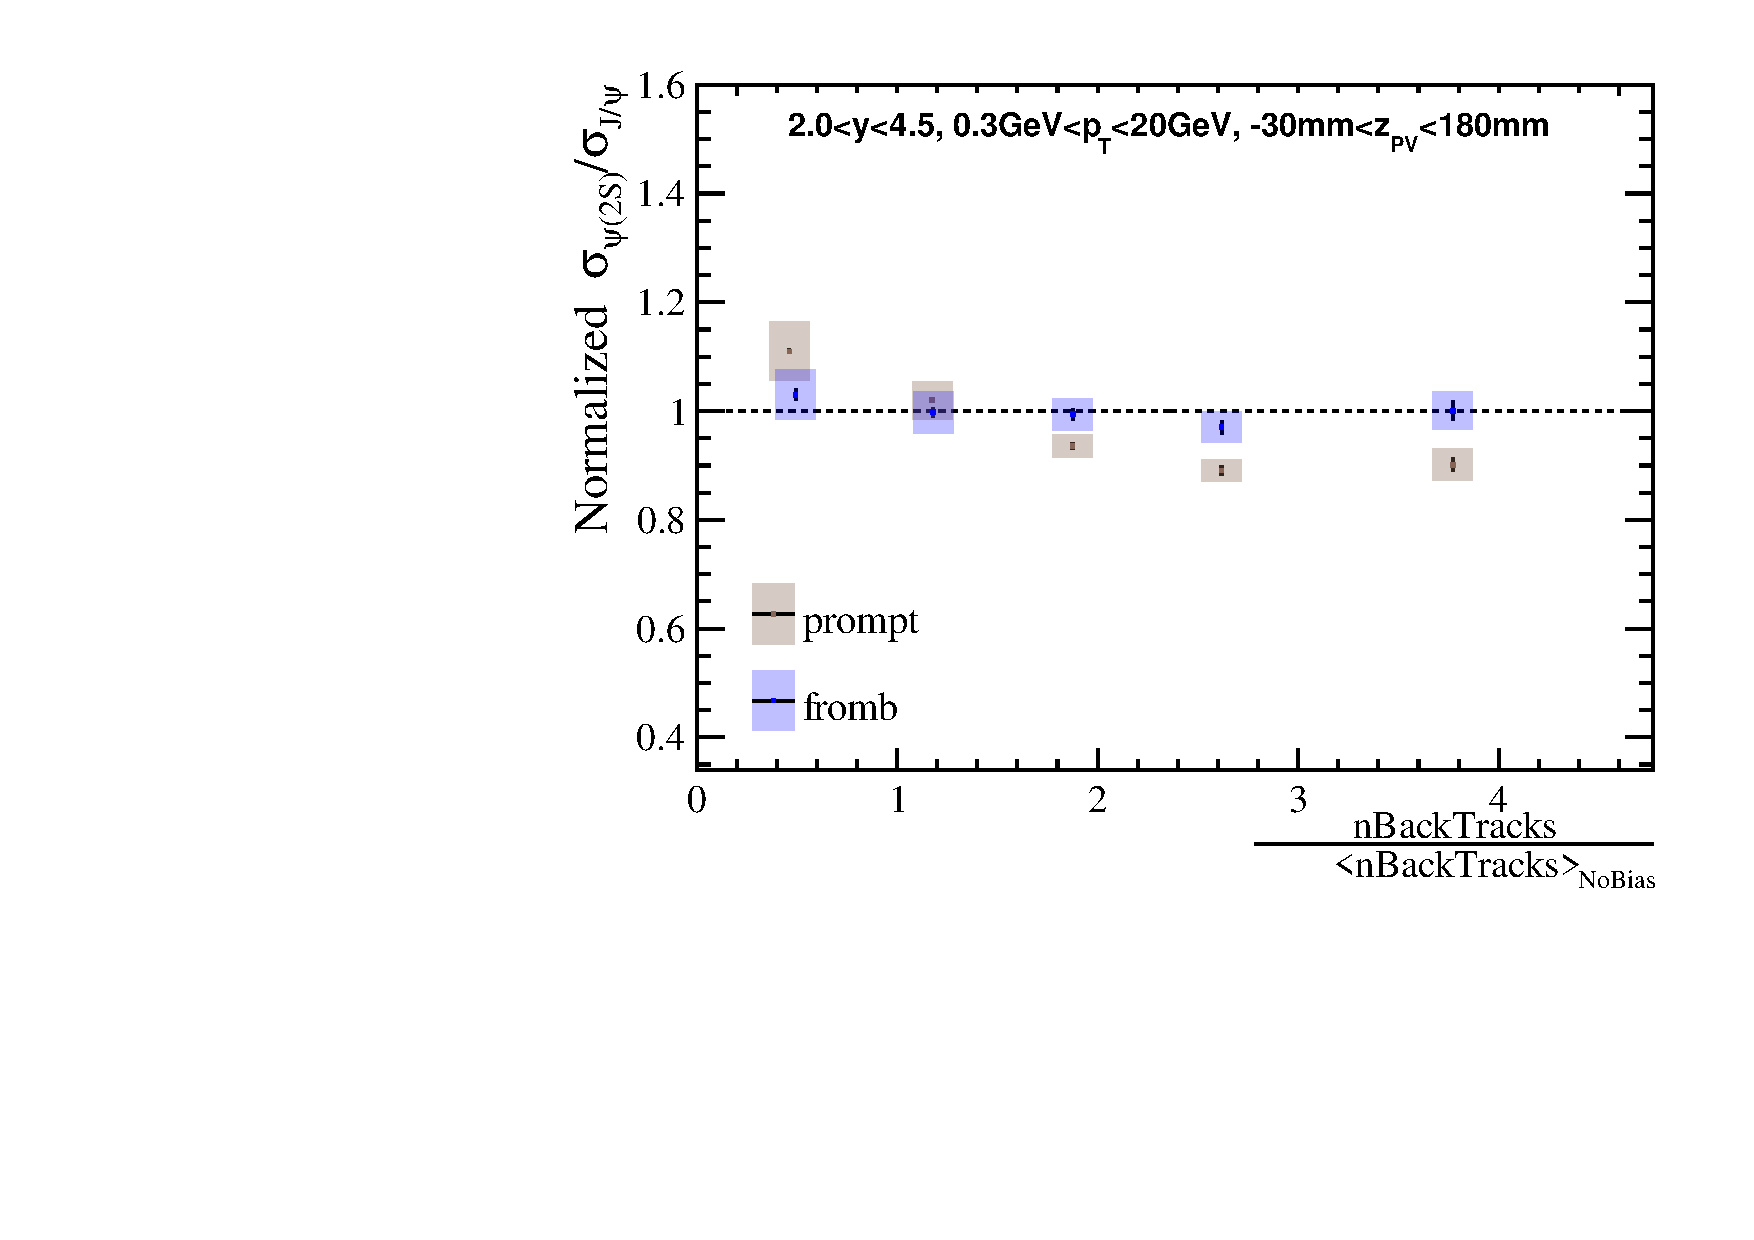
\includegraphics[width=0.49\linewidth]{pdf/Result/AllB.pdf}
    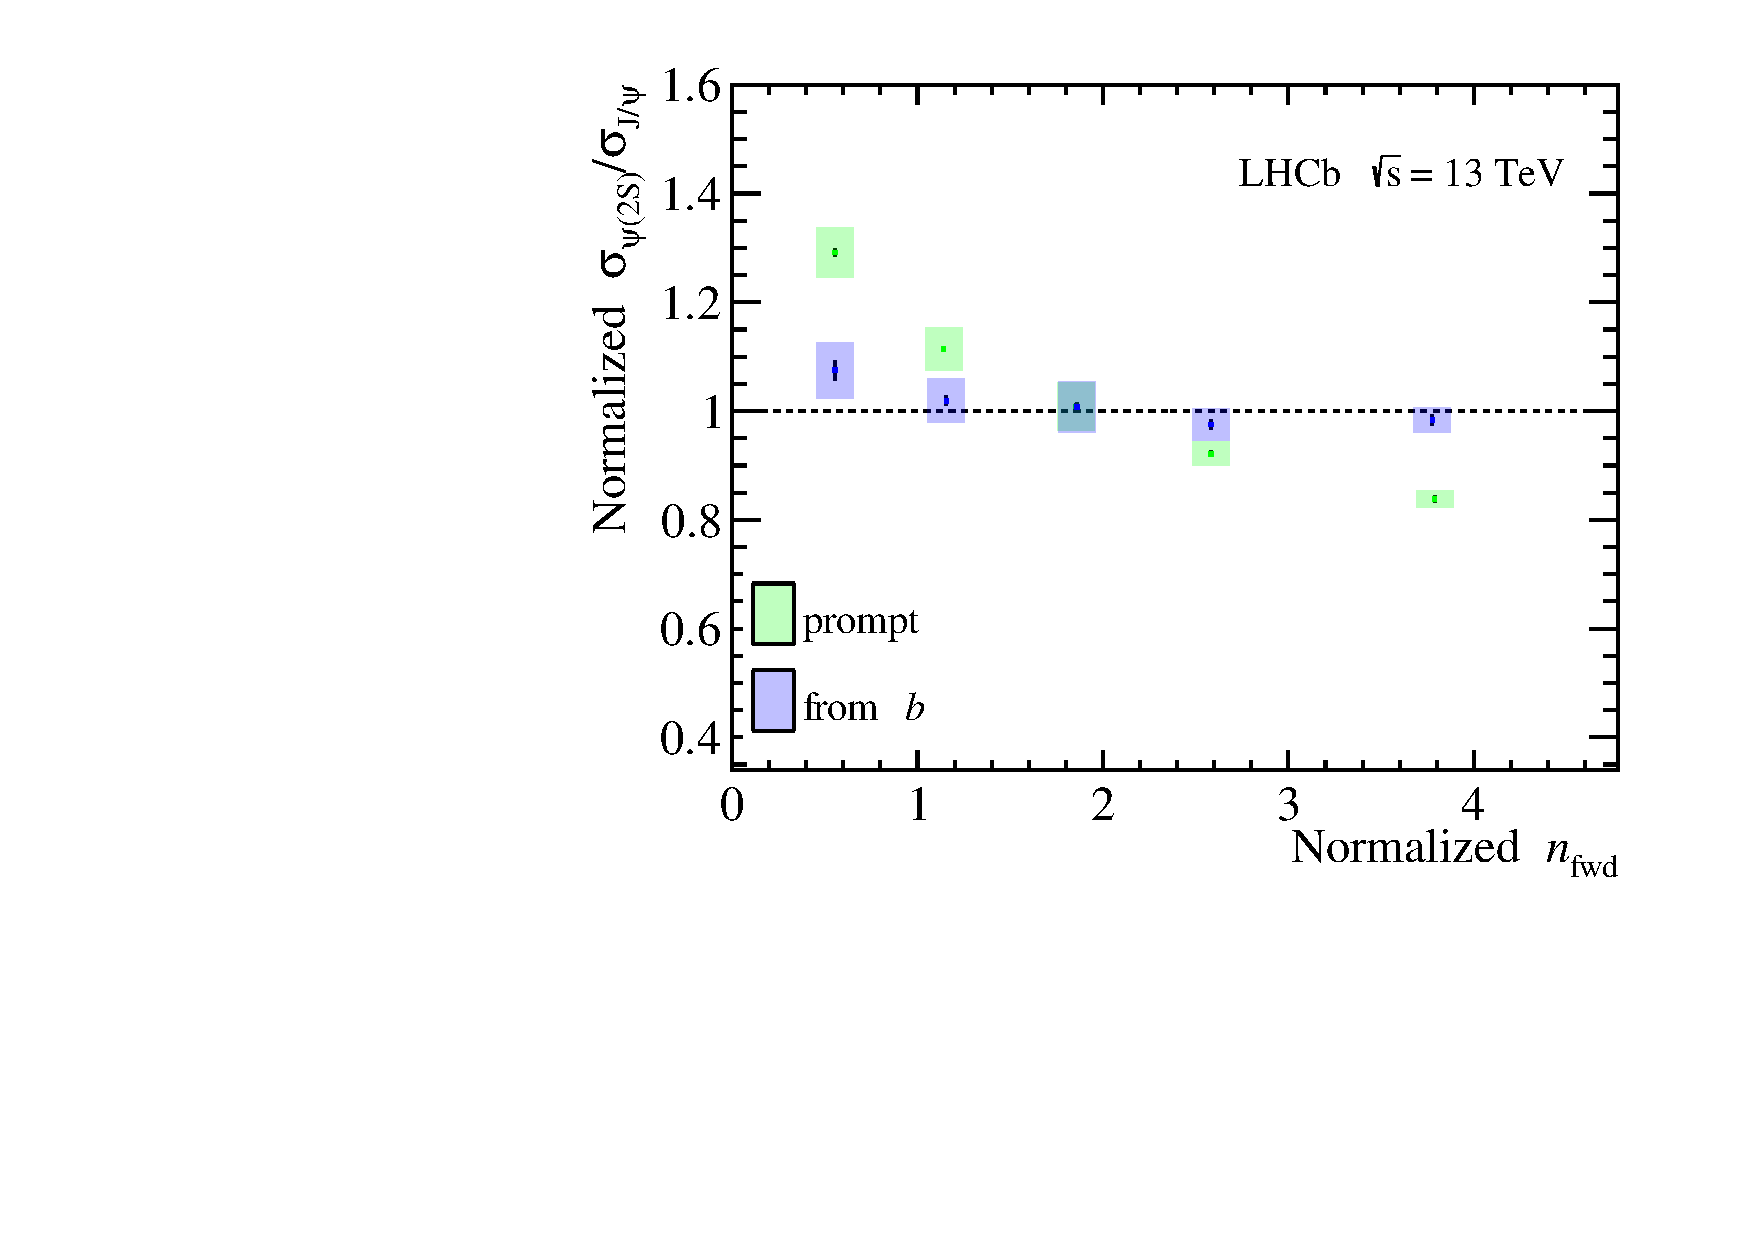
\includegraphics[width=0.49\linewidth]{pdf/Result/AllF.pdf}
    \vspace*{-0.5cm}
  \end{center}
  \caption{The ratio of integrated production over \pt-$y$ as a function of nBackTracks and nForwardTracks.
    }
  \label{RatioFB}
\end{figure}
The ratio of production from $b$-hadron decay is roughly independent of multiplicity under three different kinds of schemes. The decreasing trend for the ratio versus nBackTracks is much slower than the other two. 
This indicates that the relative suppression is correlated with the local particle multiplicity since an independent multiplicity variable leads to a slower decrease. It is within expectation since \psitwos has a larger radius and 
lower bounding energy so a preferential dissociation may happen when interacting with the co-moving matters after the collisions. Theoretically, nBackTracks is a multiplicity variable independent of the measured ratio, and the ratio should roughly be the same in different multiplicity regions. But nBackTracks is not fully independent since there is a correlation between nForwardTracks and nBackTracks with a correlation factor of 0.54 for \jpsi and 0.51 for \psitwos.
To study the effect produced by the correlation between nBackTracks and nForwardTracks, we measure the mean values of nForwardTracks in each nBackTracks bin for both prompt \jpsi and \psitwos. Then we follow the procedures in Sec~\ref{sec:binCorr} to calculate the x-coordinates of nForwardTracks in each nBackTracks bin. Finally, the normalized ratios in different nBackTracks bin is migrated to the plot of nForwardTracks in Figs.~\ref{BtoF}. We find a good agreement on the decreasing trend, which means the dependence of normalized \psitwos-to-\jpsi ratio on nBackTracks could result from the correlation between nBackTracks and nForwardTracks.
\begin{figure}[H] 
    \begin{center}
      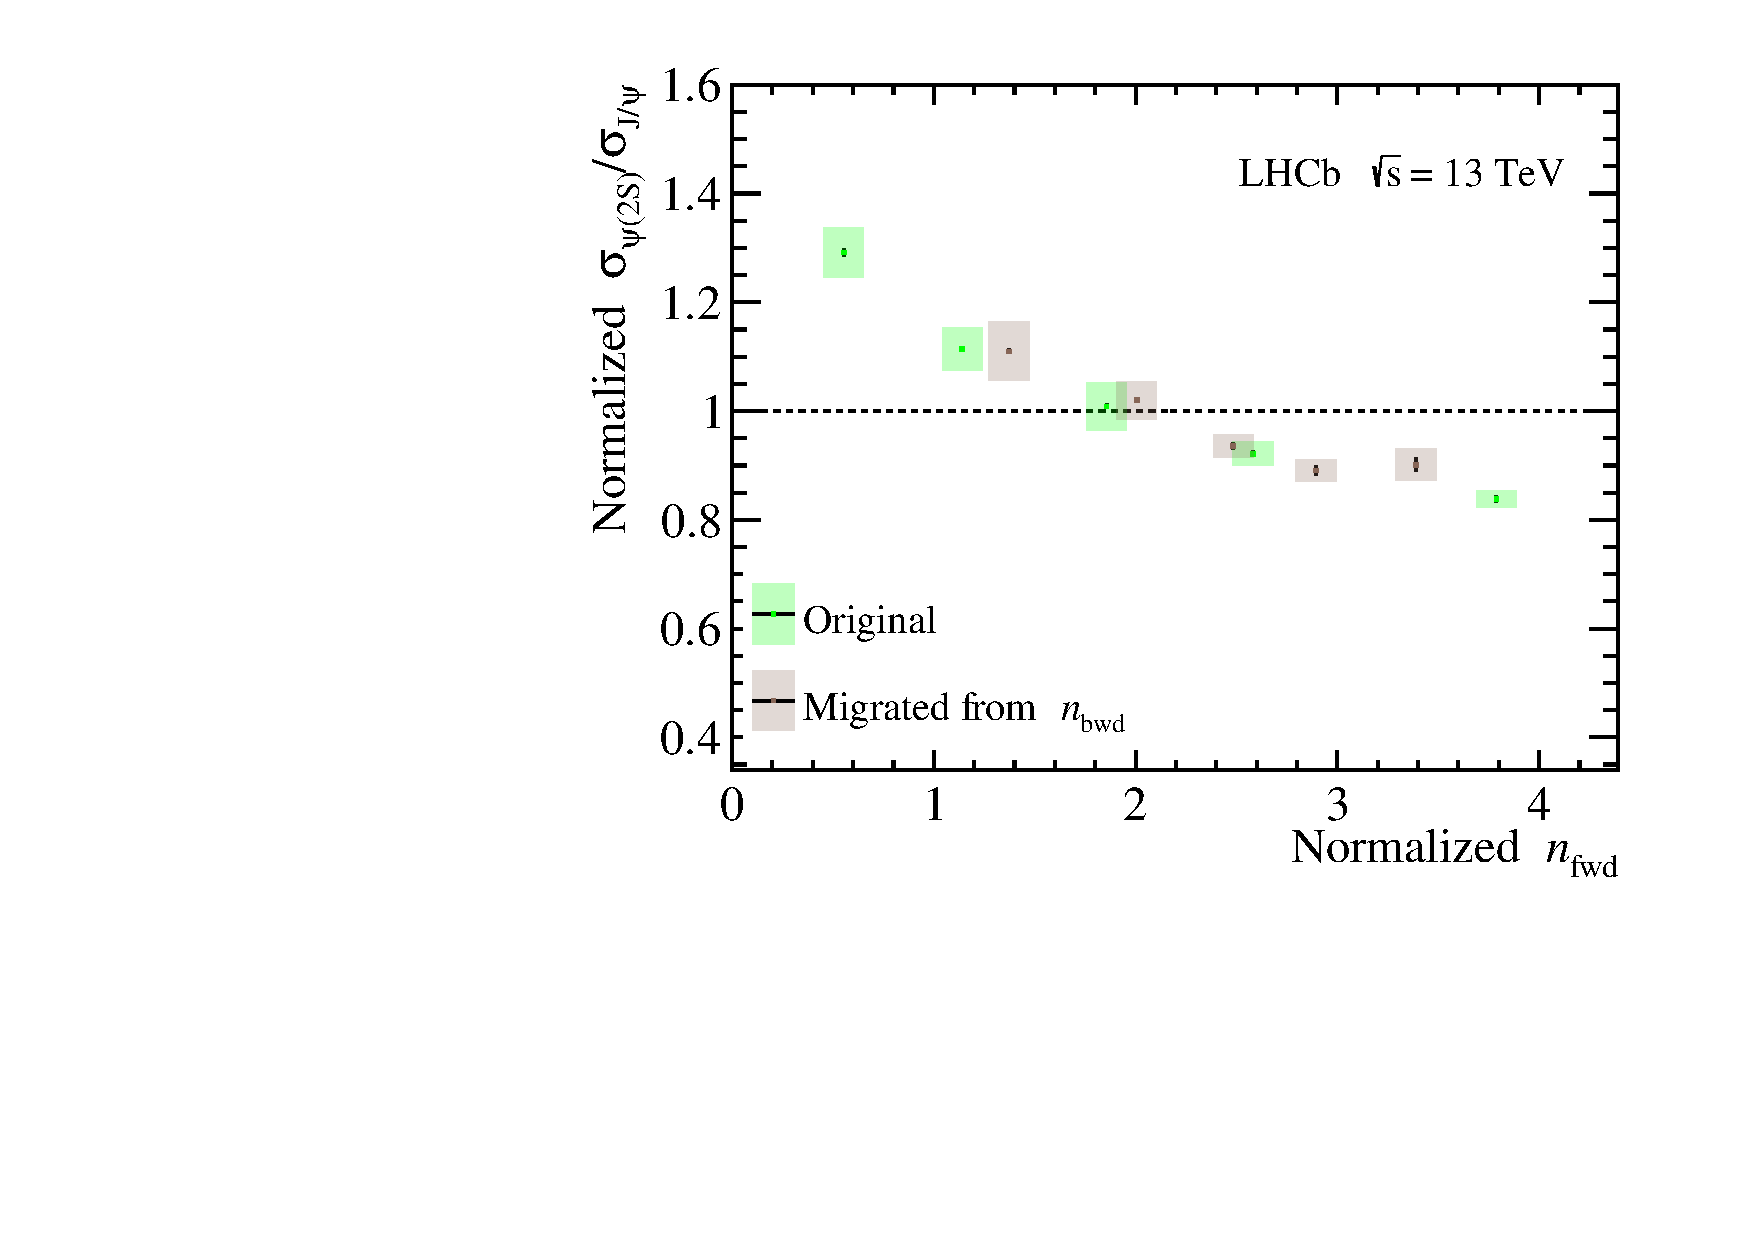
\includegraphics[width=0.8\linewidth]{pdf/Result/AllBtoF.pdf}
    \end{center}
    \caption{ Data points on nBackTracks are migrated to plot of nForwardTracks by find the mean value of nForwardTracks in each nBackTracks bin.
      } 
    \label{BtoF}
\end{figure}
\subsection{\psitwos-to-\jpsi ratio in different \pt regions}
In Sec~\ref{sec:binCorr} we have discussed how to find appropriate horizontal coordinates for the \psitwos-to-\jpsi ratio in $2.0<y<4.5$ and $0.3\gevc<\pt<20\gevc$. The multiplicity distributions in different \pt ranges are significantly different. Hence, for all the results in different \pt ranges, we need to repeat the procedures in Sec~\ref{sec:binCorr} to find appropriate horizontal coordinates for plotting. And the final results in different \pt ranges are shown in Fig~\ref{RatioPT_PVN}, Fig~\ref{RatioPT_For} and Fig~\ref{RatioPT_Back}. In three binning schemes for multiplicity, the ratios share the same property that, in low \pt region, the preferential suppression of \psitwos is higher than that in higher \pt region.
\begin{figure}[H]
  \begin{center}
	  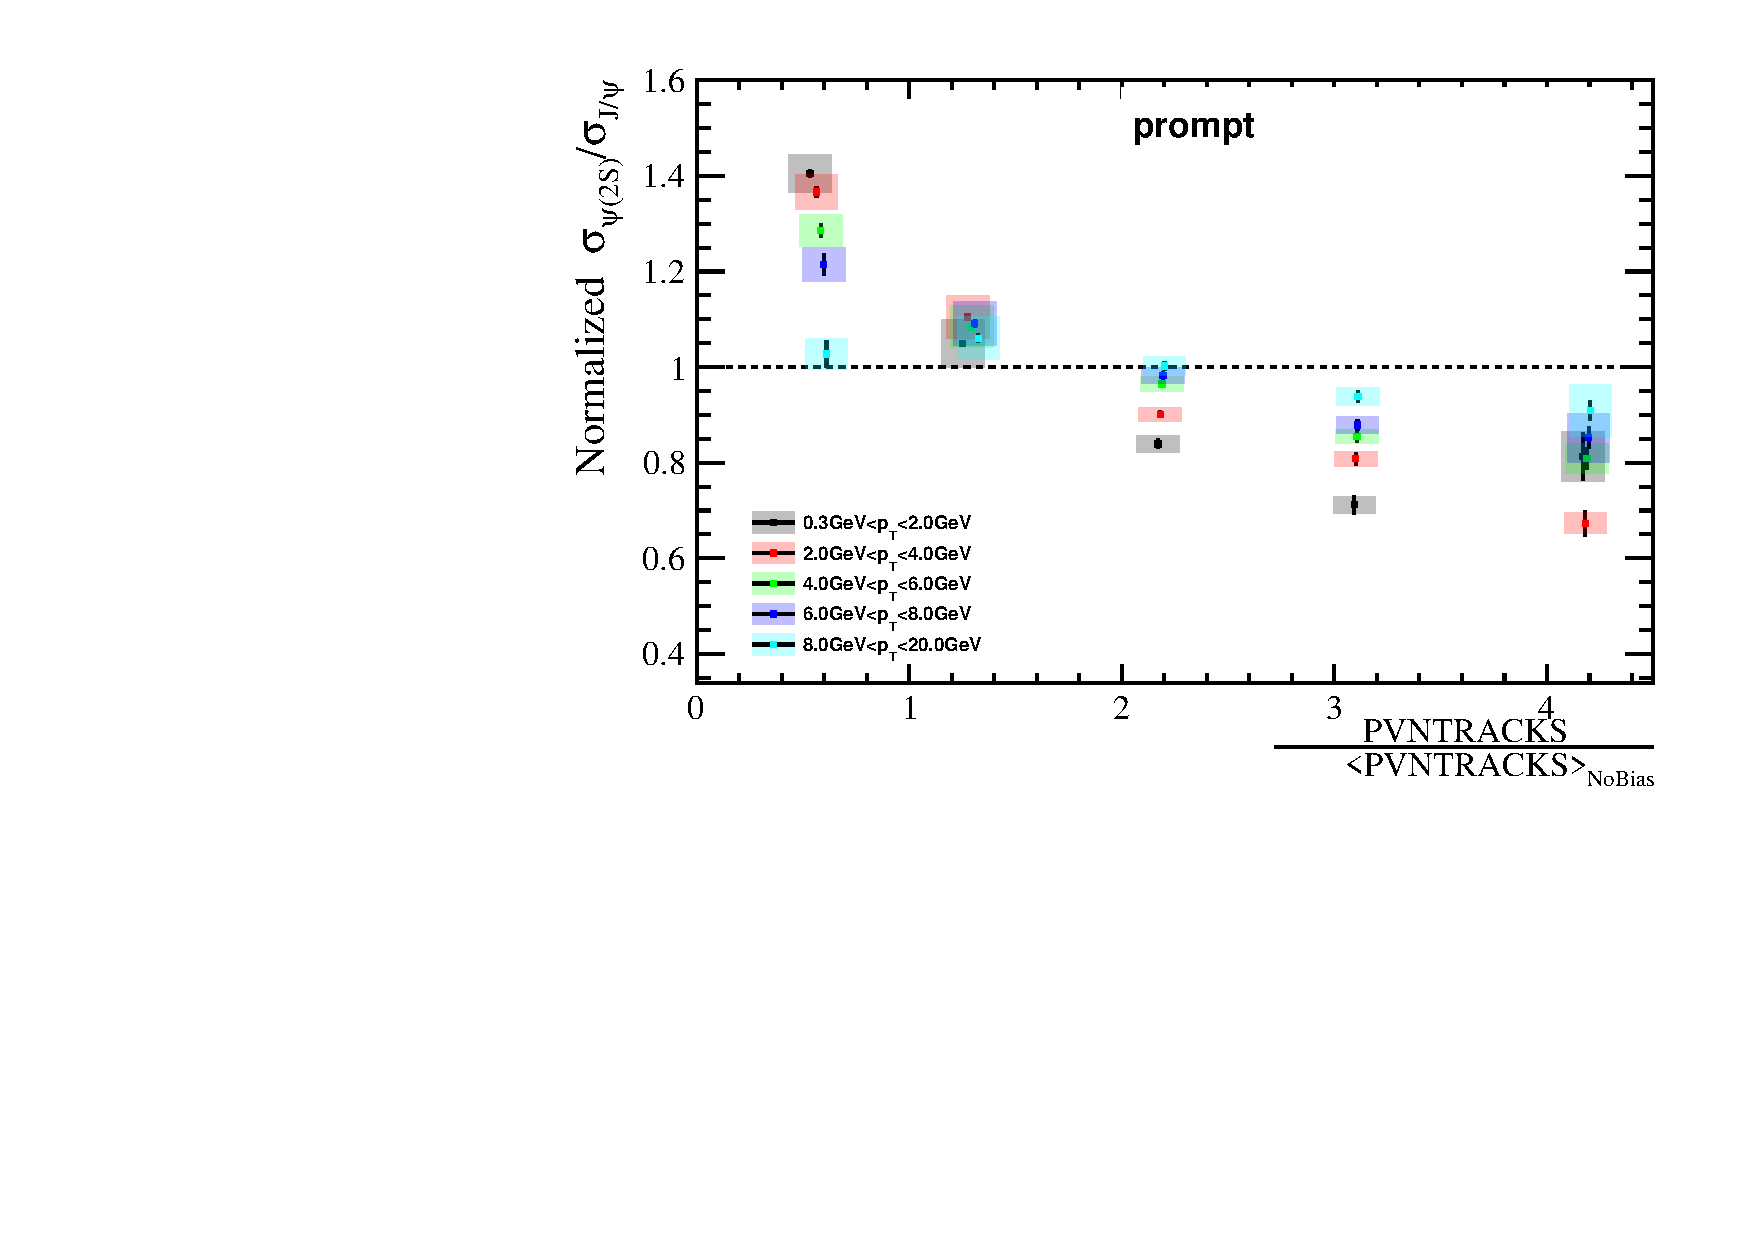
\includegraphics[width=0.48\linewidth]{pdf/Result/promptRatioPT.pdf}
    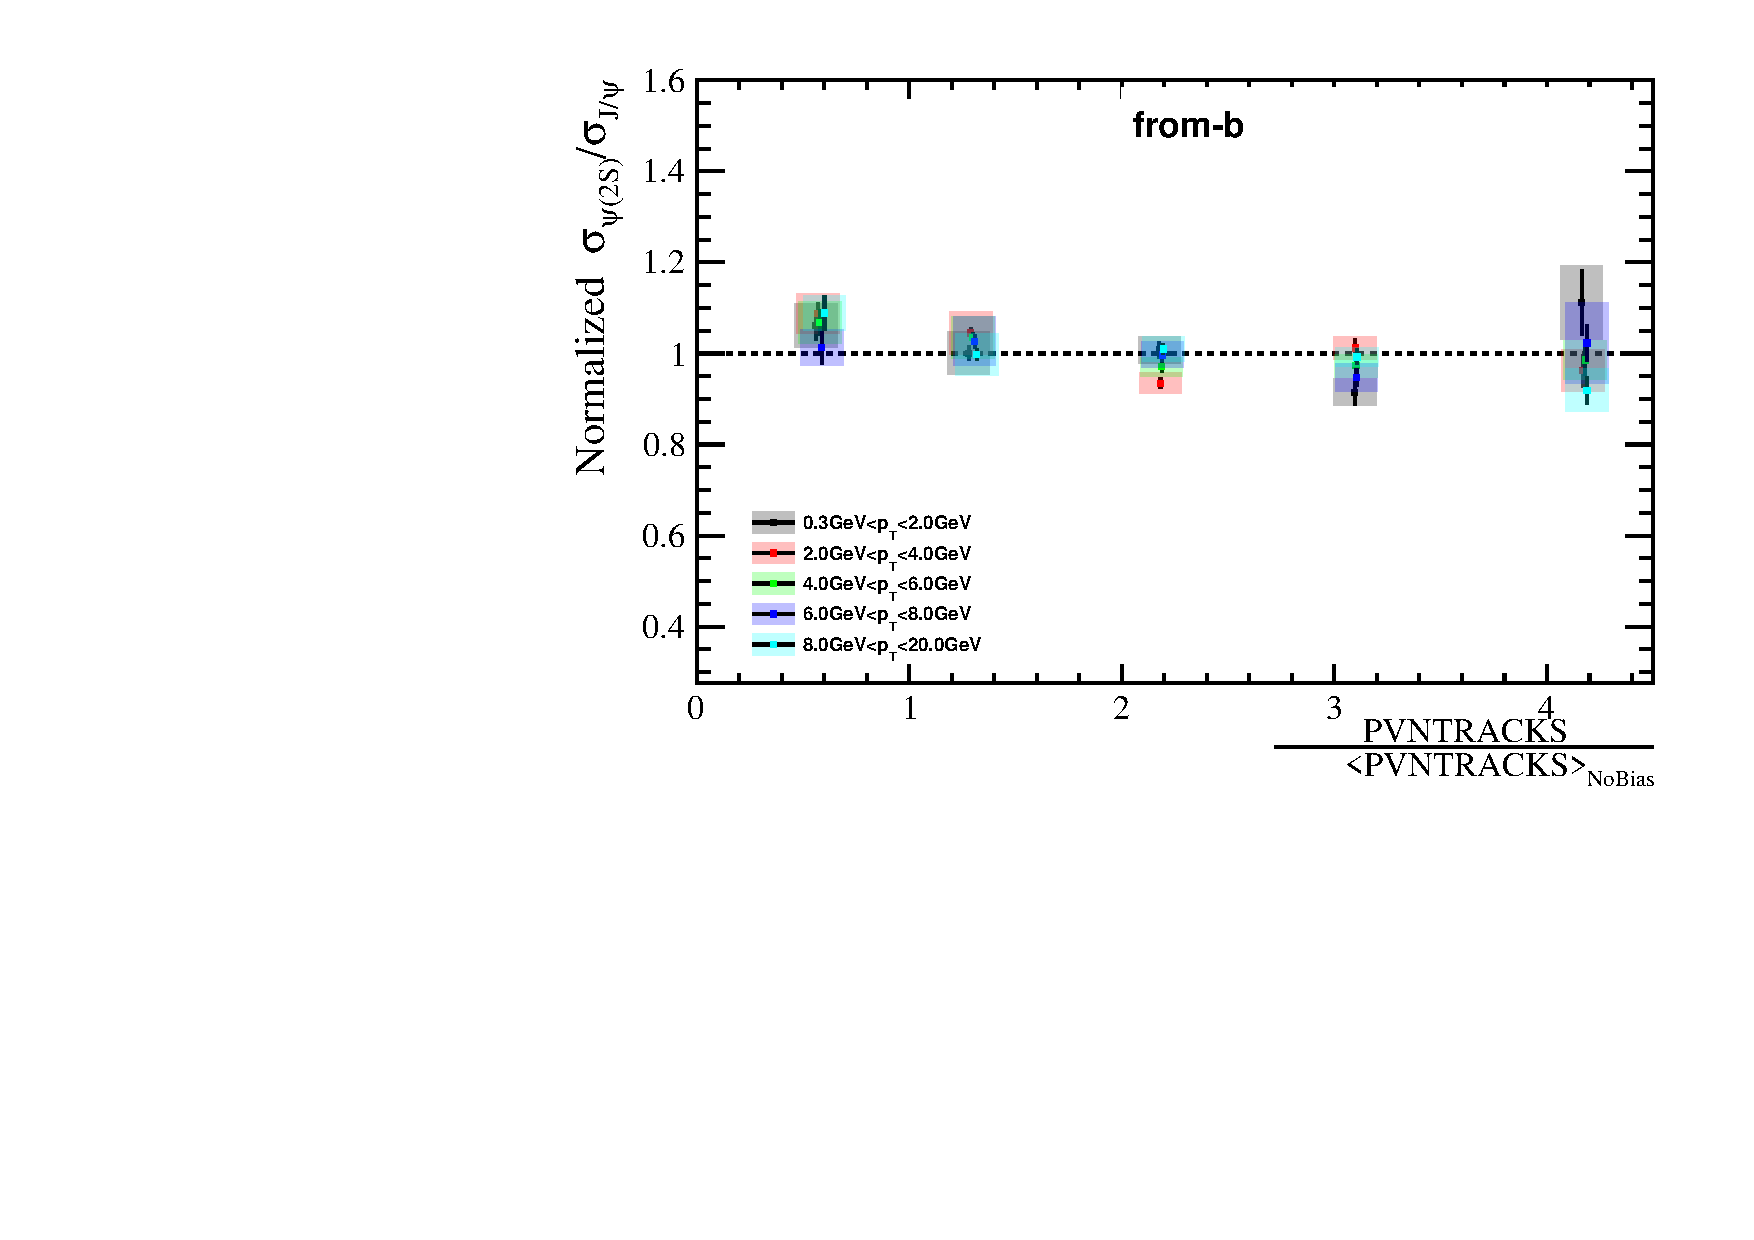
\includegraphics[width=0.48\linewidth]{pdf/Result/frombRatioPT.pdf}
  \end{center}
  \caption{Ratio of \psitwos to \jpsi in different \pt region when multiplicity is divided in PVNTRACKS}.
  \label{RatioPT_PVN}
\end{figure}
\begin{figure}[H]
  \begin{center}
    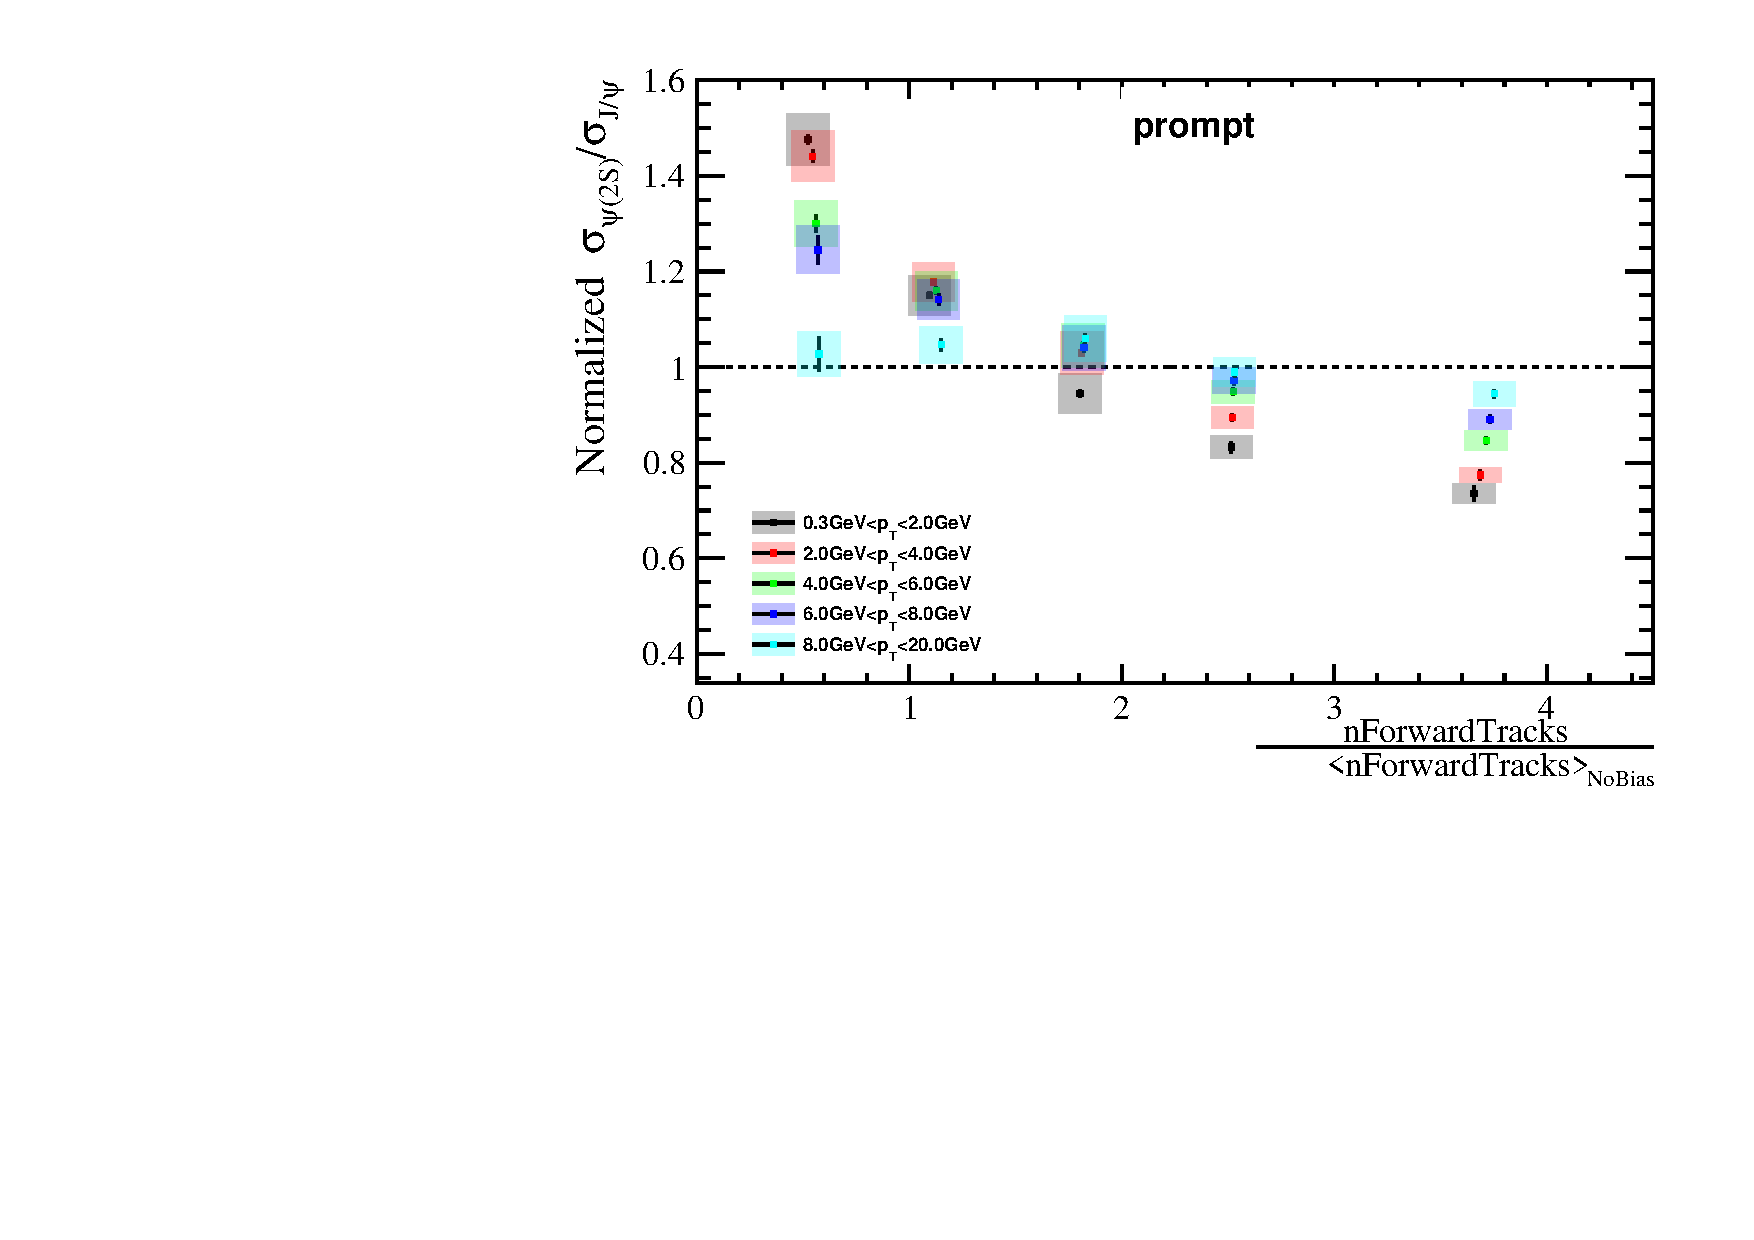
\includegraphics[width=0.48\linewidth]{pdf/Result/promptRatioPTF.pdf}
    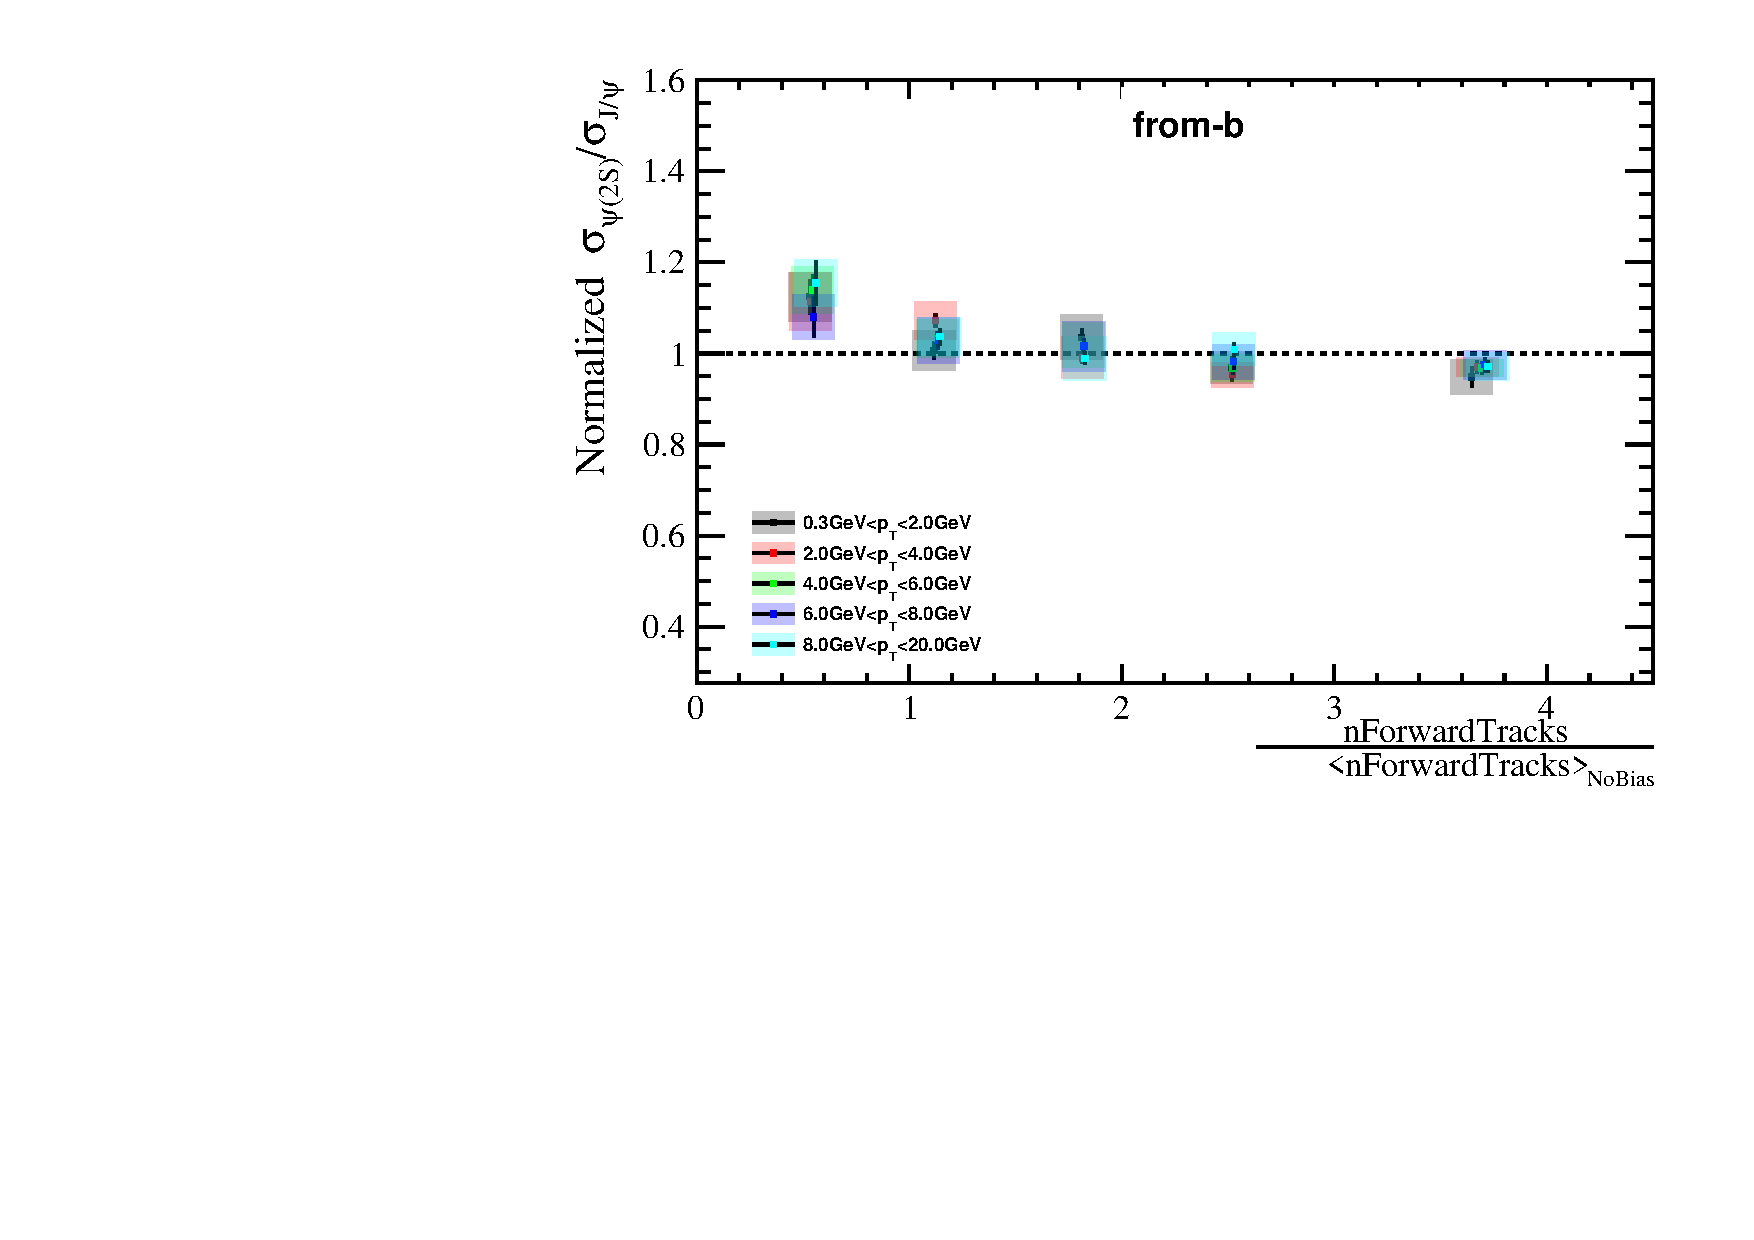
\includegraphics[width=0.48\linewidth]{pdf/Result/frombRatioPTF.pdf}
  \end{center}
  \caption{Ratio of \psitwos to \jpsi in different \pt region when multiplicity is divided in nForwardTracks}.
  \label{RatioPT_For}
\end{figure}
\begin{figure}[H]
  \begin{center}
    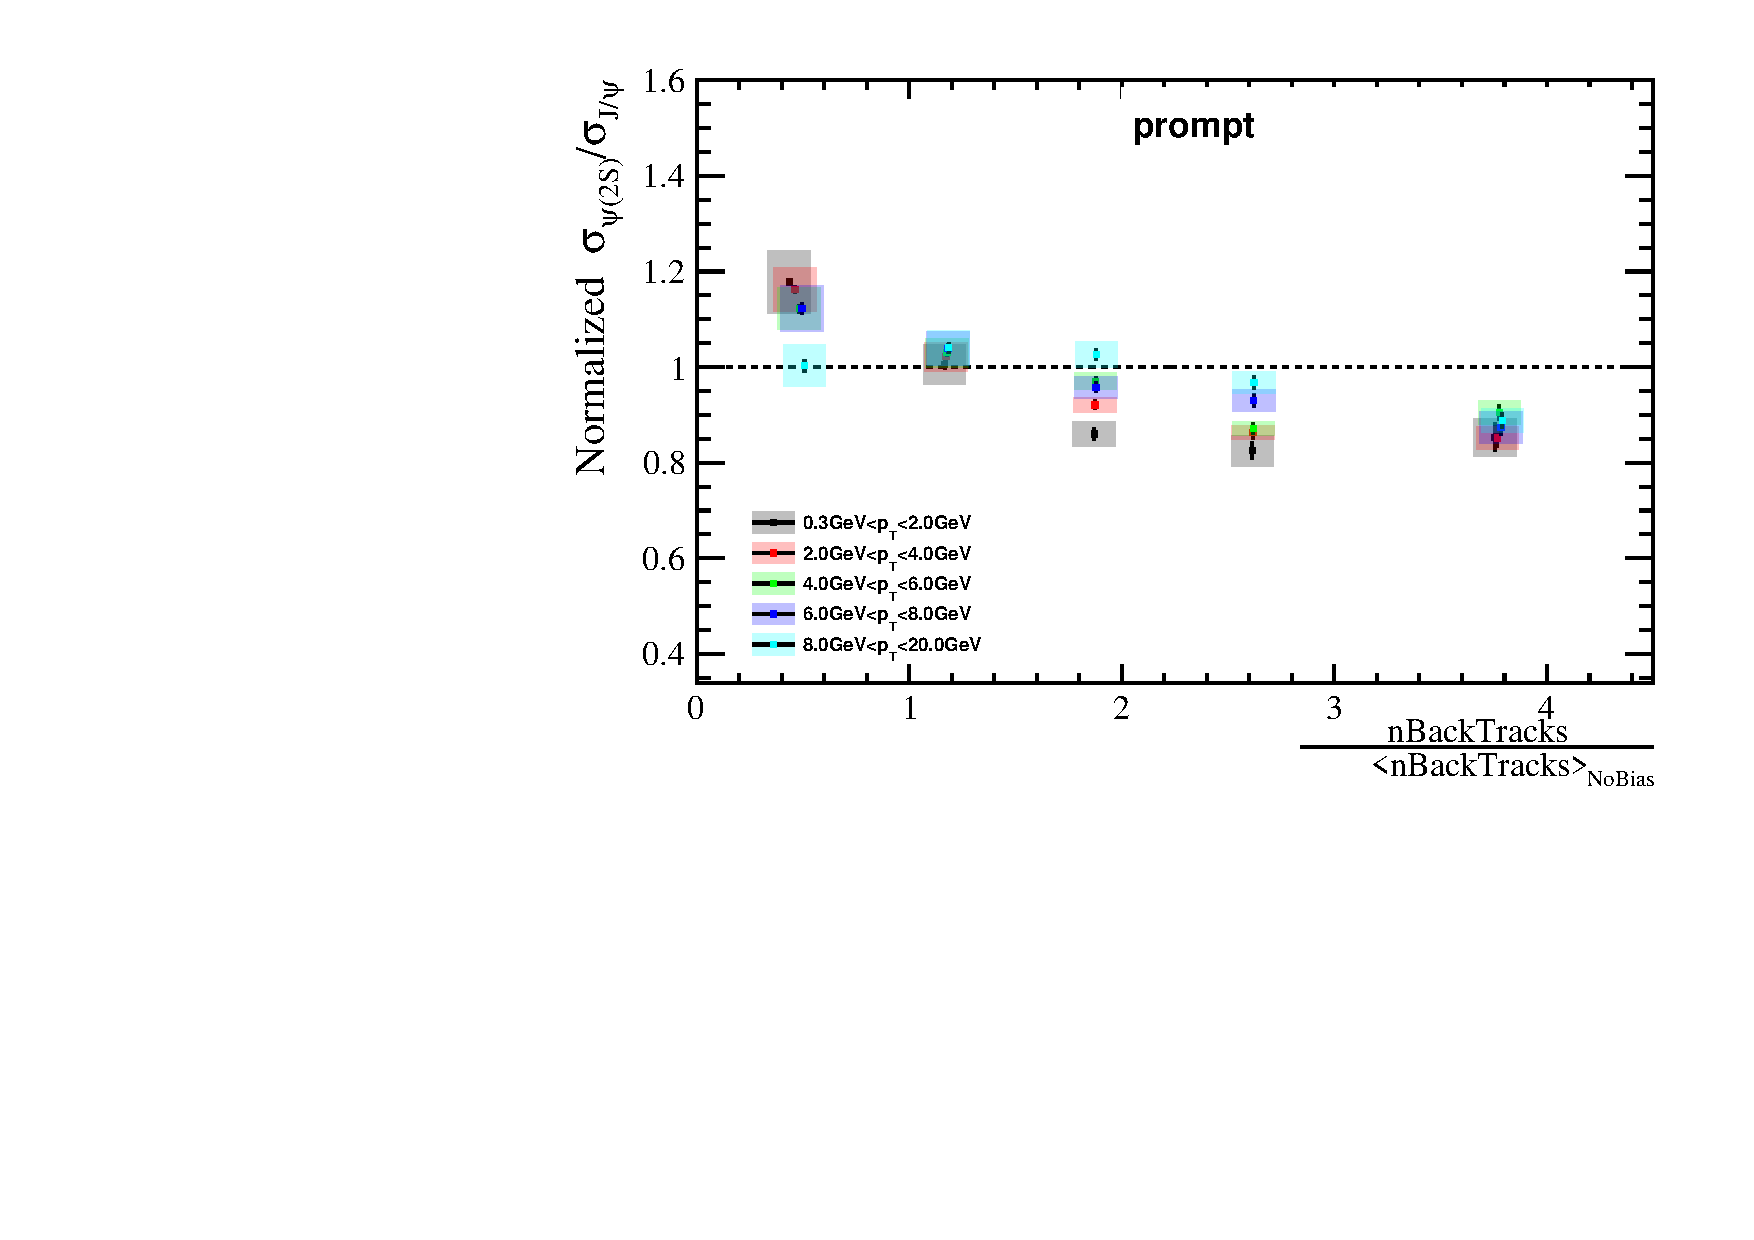
\includegraphics[width=0.48\linewidth]{pdf/Result/promptRatioPTB.pdf}
    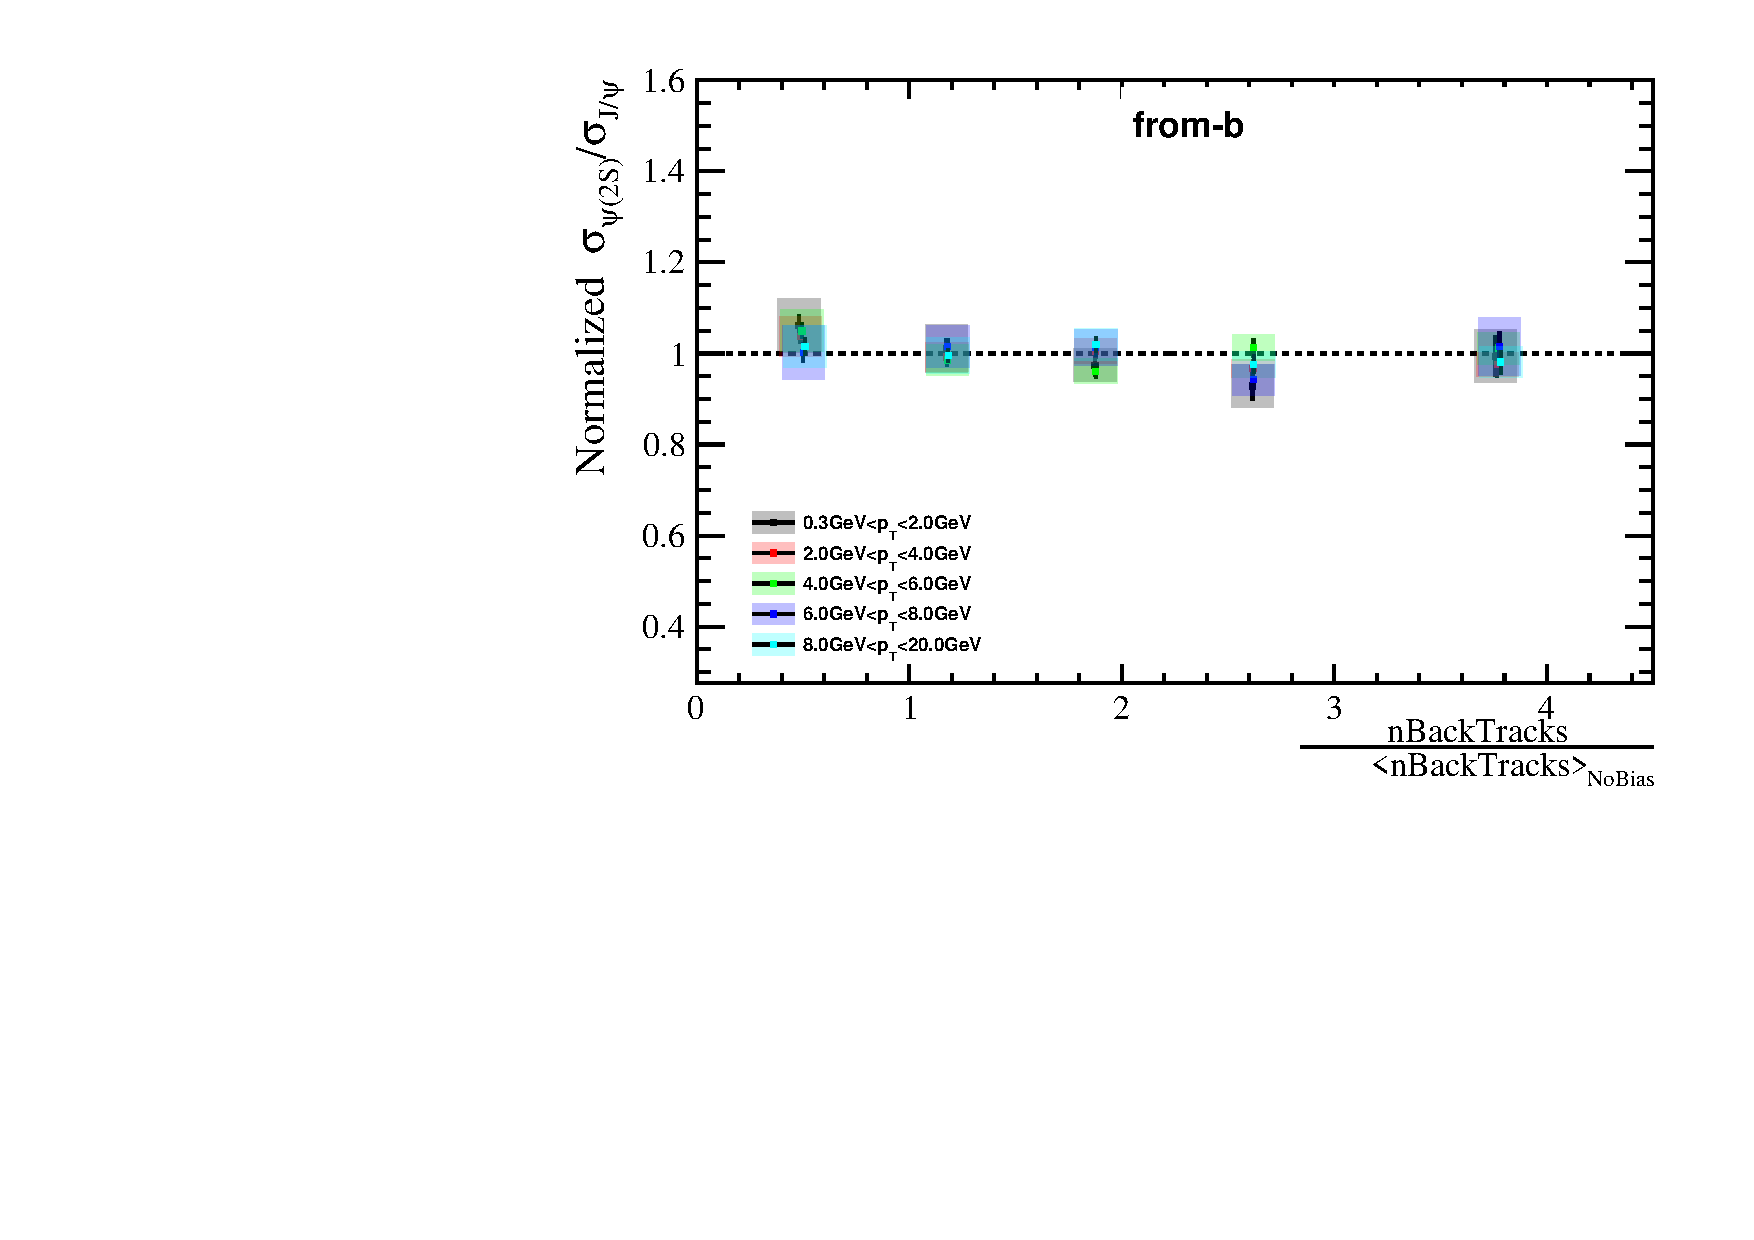
\includegraphics[width=0.48\linewidth]{pdf/Result/frombRatioPTB.pdf}
  \end{center}
  \caption{Ratio of \psitwos to \jpsi in different \pt region when multiplicity is divided in nBackTracks}.
  \label{RatioPT_Back}
\end{figure}
\subsection{\psitwos-to-\jpsi ratio in different $y$ regions}
The results for ratio in different rapidity bins are given in Figs~\ref{RatioY} when taking PVNTRACKS as a multiplicity variable. And the results for nForwardTracks and nBackTracks are given in Figs~\ref{RatioY_For} and Figs~\ref{RatioY_Back}. The results show that there is no significant difference in different rapidity regions, for both prompt and non-prompt signals.
\begin{figure}[H]
  \begin{center}
    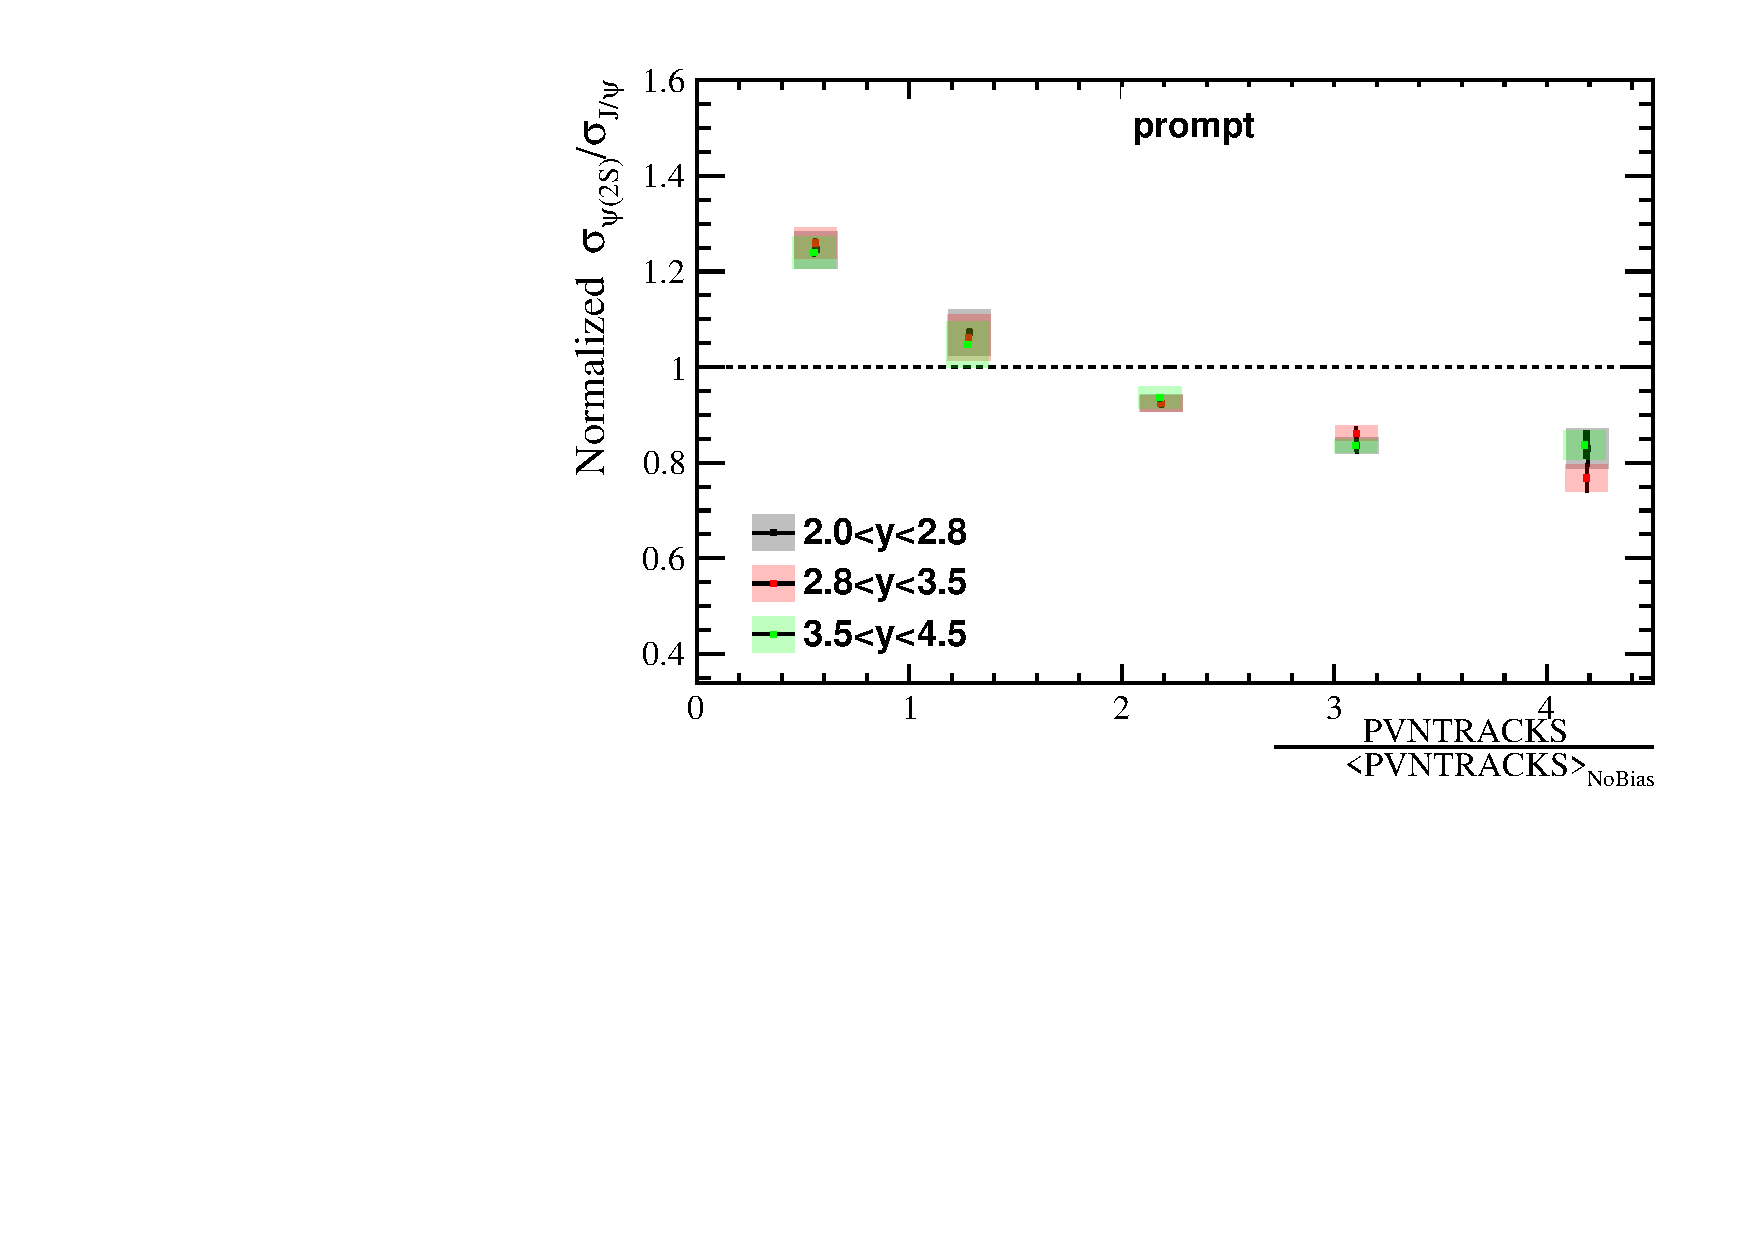
\includegraphics[width=0.48\linewidth]{pdf/Result/promptRatioY.pdf}
    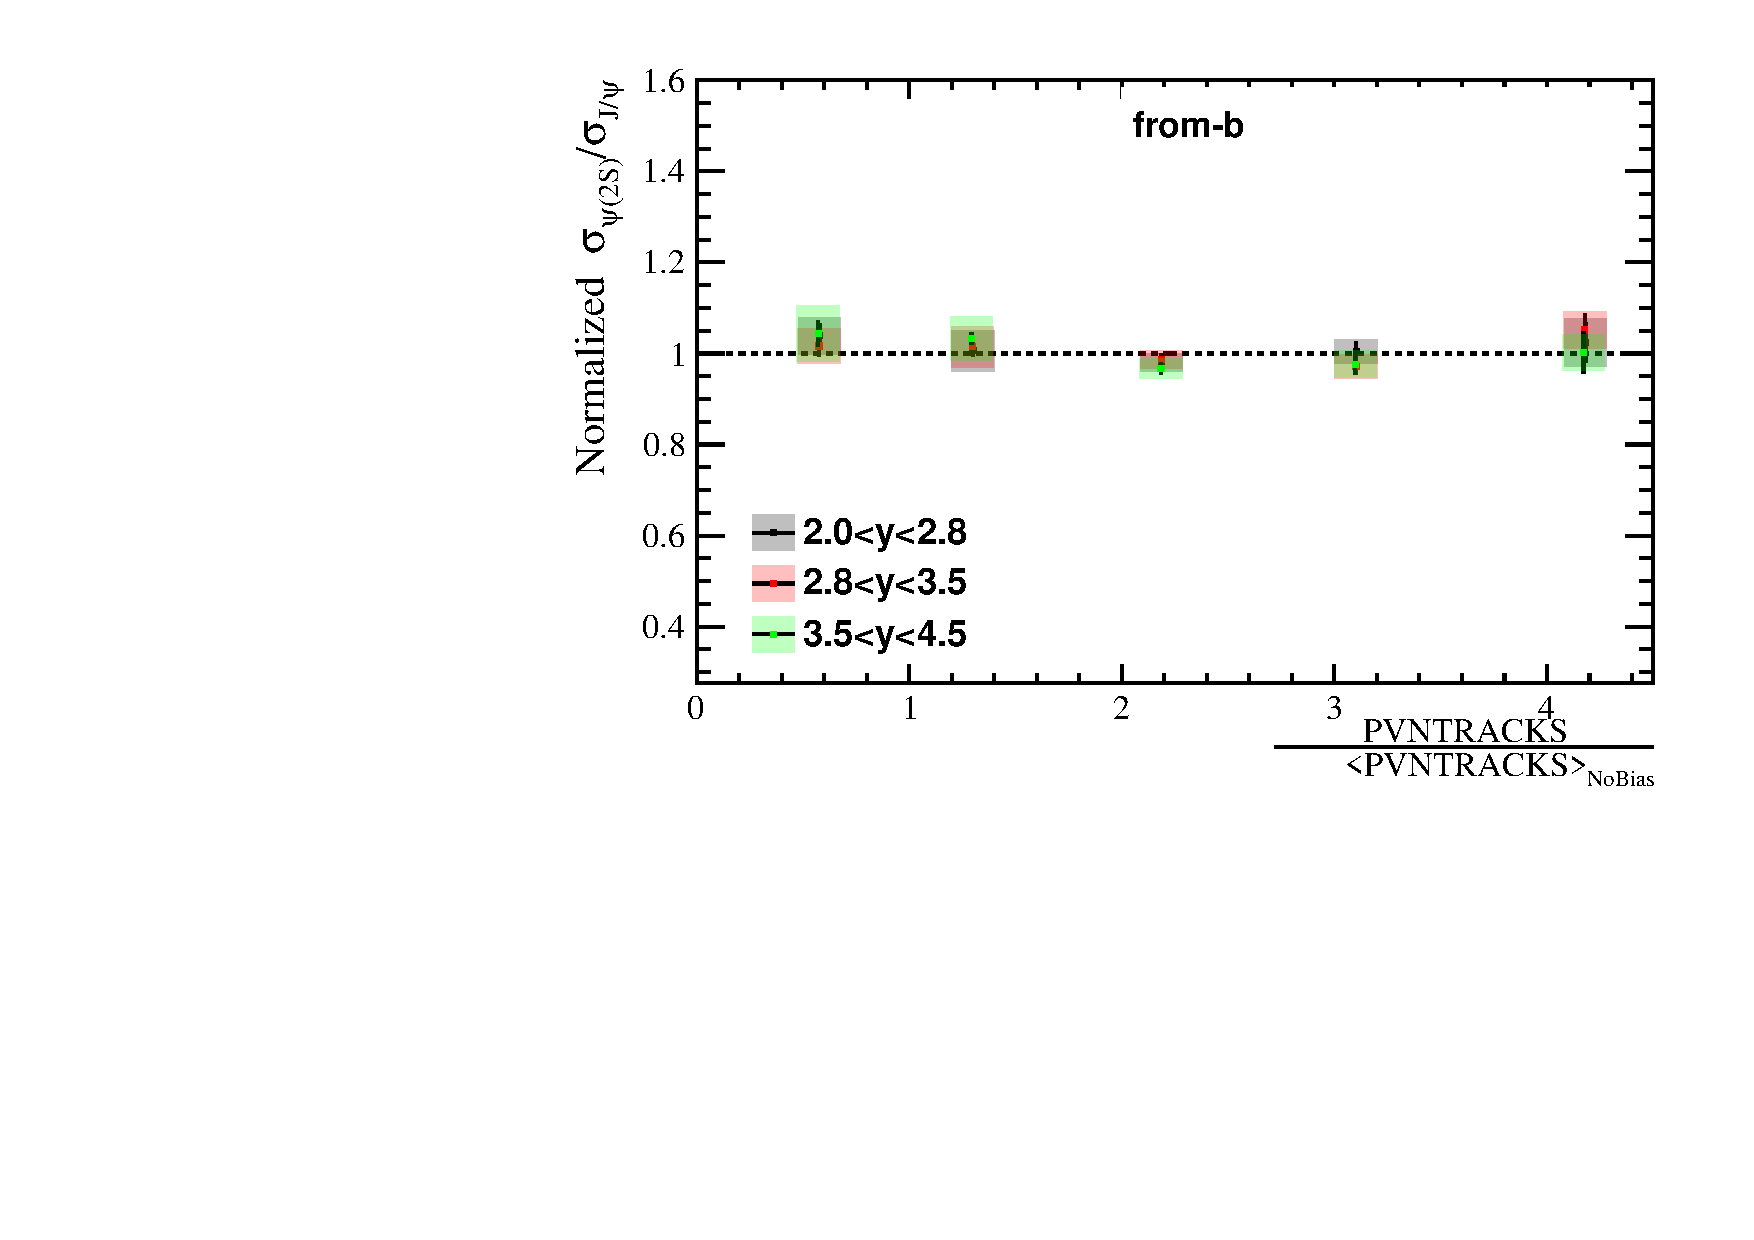
\includegraphics[width=0.48\linewidth]{pdf/Result/frombRatioY.pdf}
  \end{center}
  \caption{Ratio of \psitwos to \jpsi in different $y$ region when multiplicity is divided in PVNTRACKS}.
  \label{RatioY}
\end{figure}

\begin{figure}[H]
  \begin{center}
    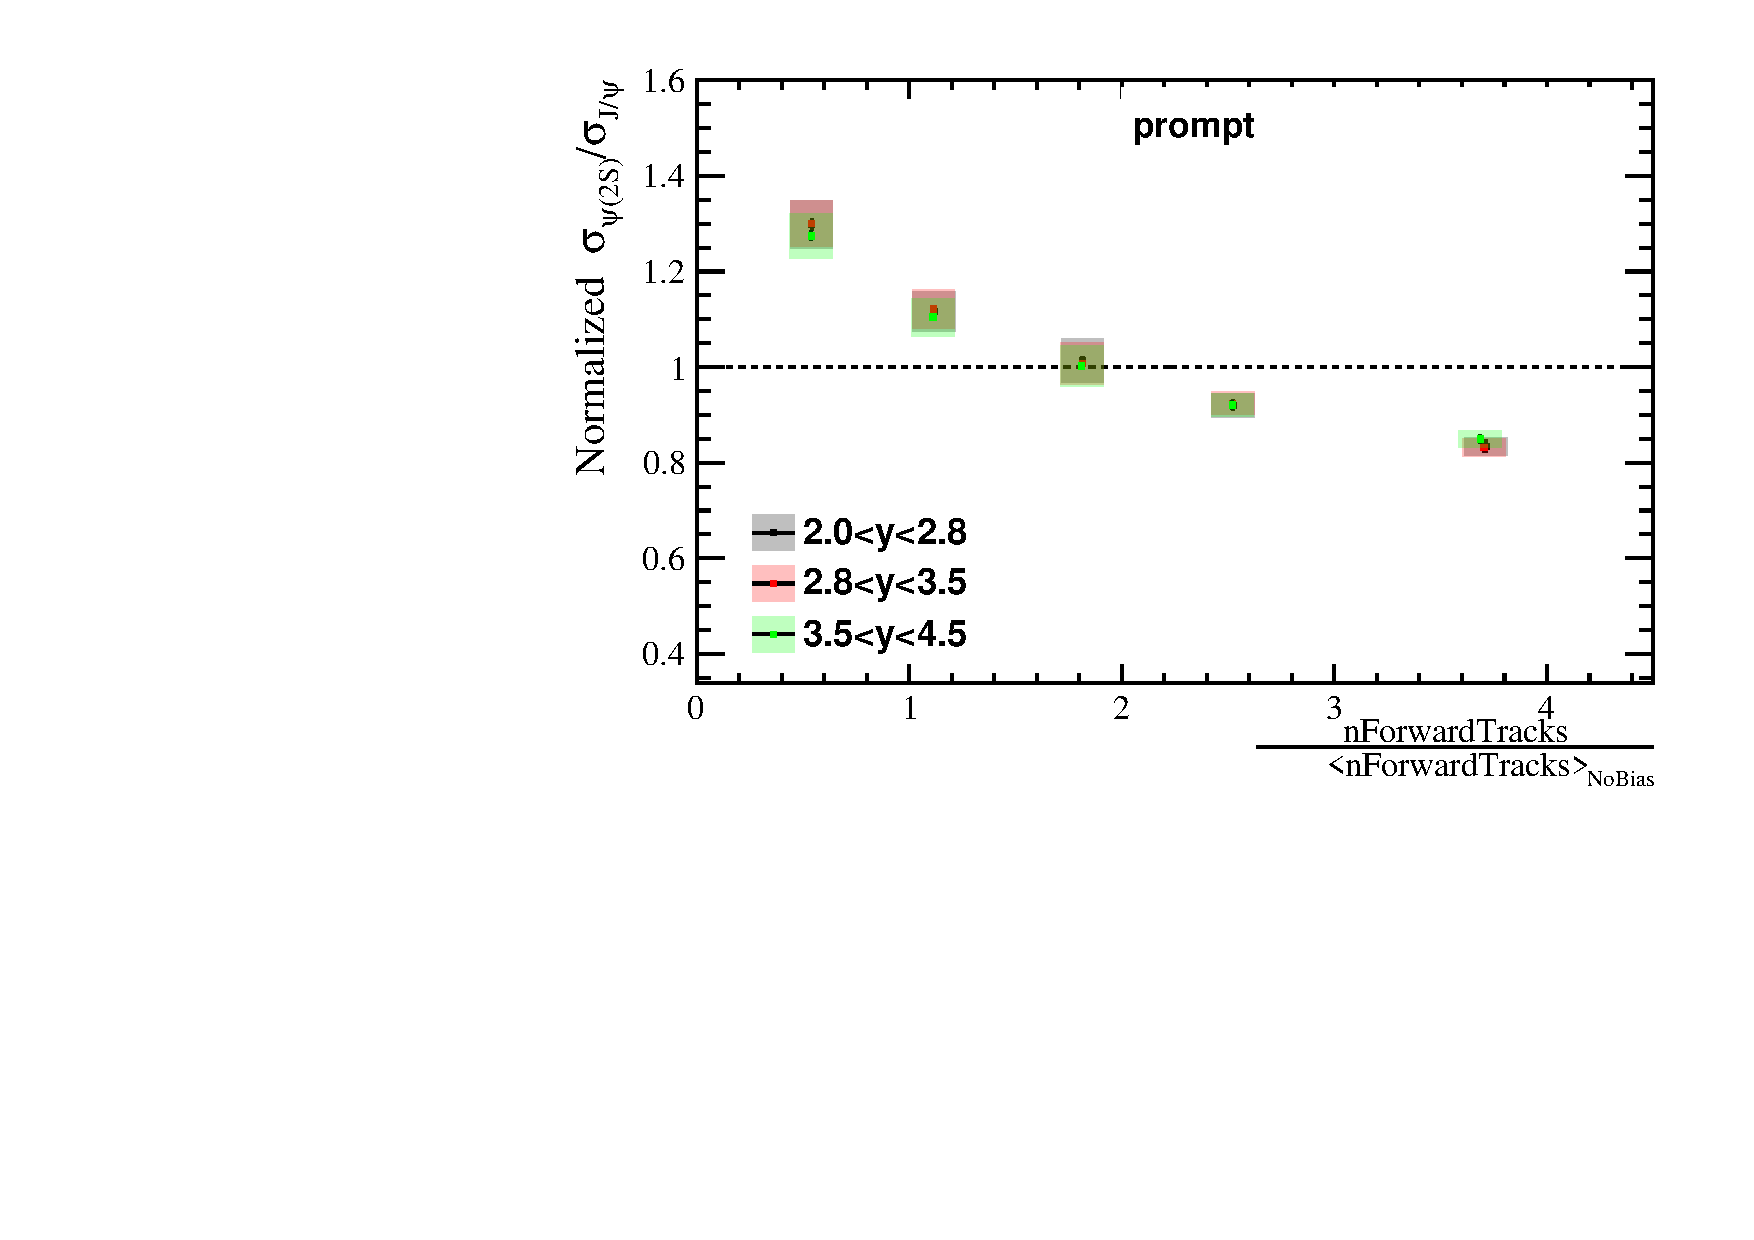
\includegraphics[width=0.48\linewidth]{pdf/Result/promptRatioYF.pdf}
    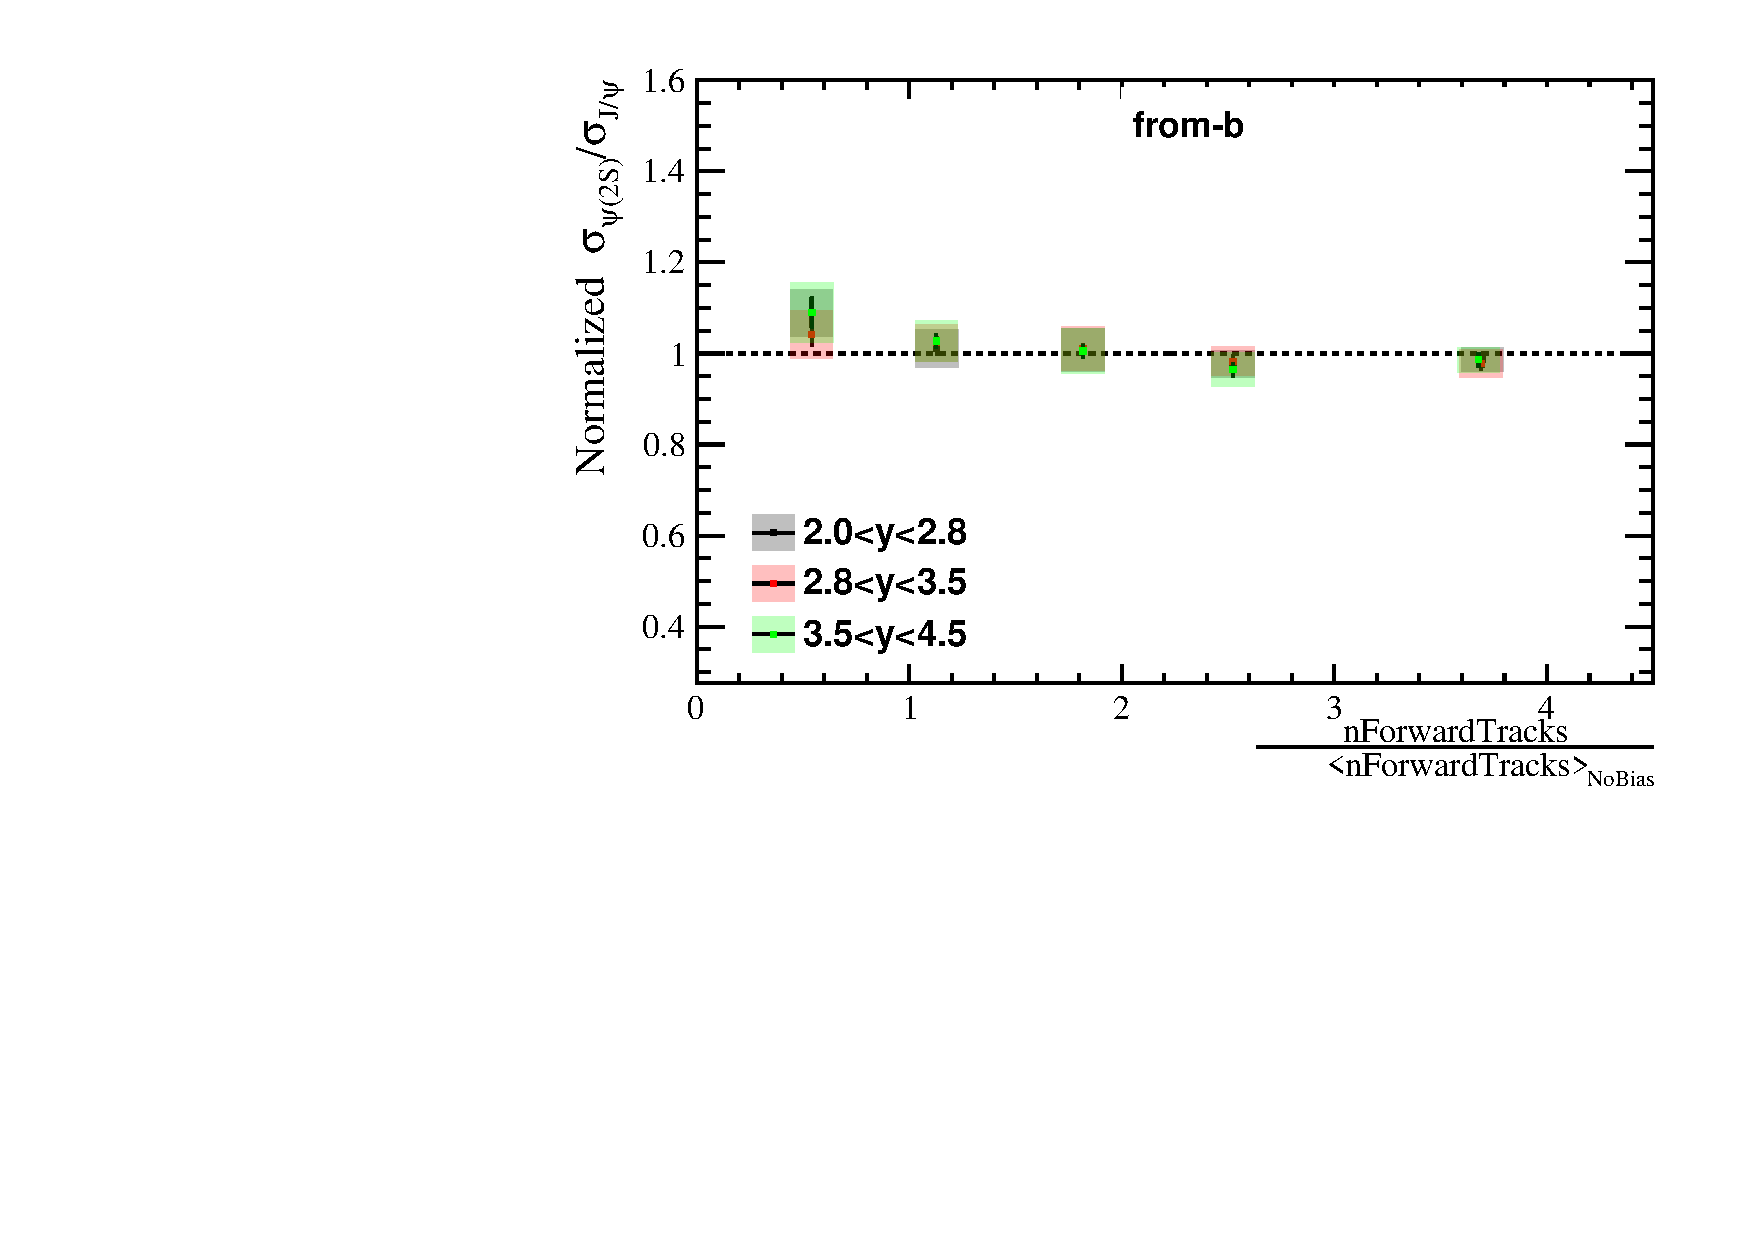
\includegraphics[width=0.48\linewidth]{pdf/Result/frombRatioYF.pdf}
  \end{center}
  \caption{Ratio of \psitwos to \jpsi in different $y$ region when multiplicity is divided in nForwardTracks}.
  \label{RatioY_For}
\end{figure}

\begin{figure}[H]
  \begin{center}
    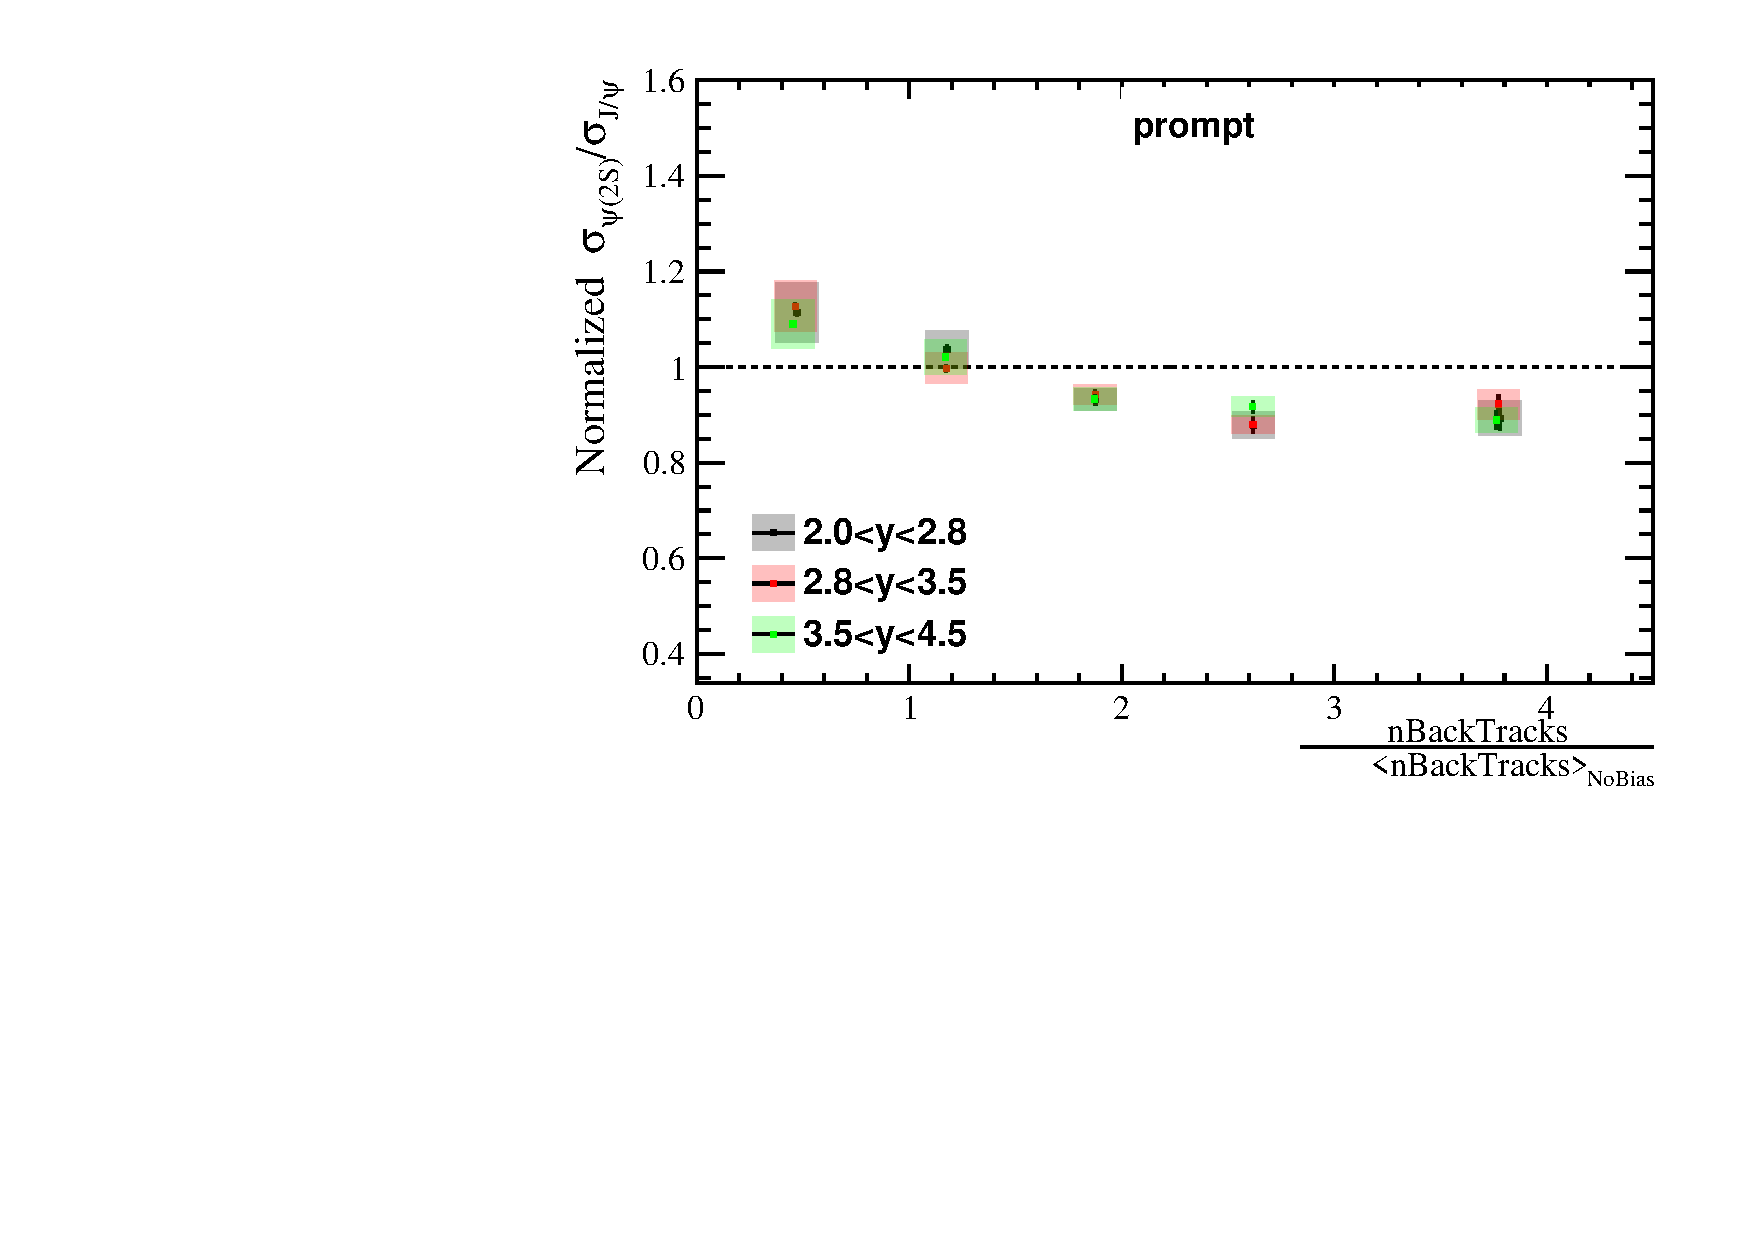
\includegraphics[width=0.48\linewidth]{pdf/Result/promptRatioYB.pdf}
    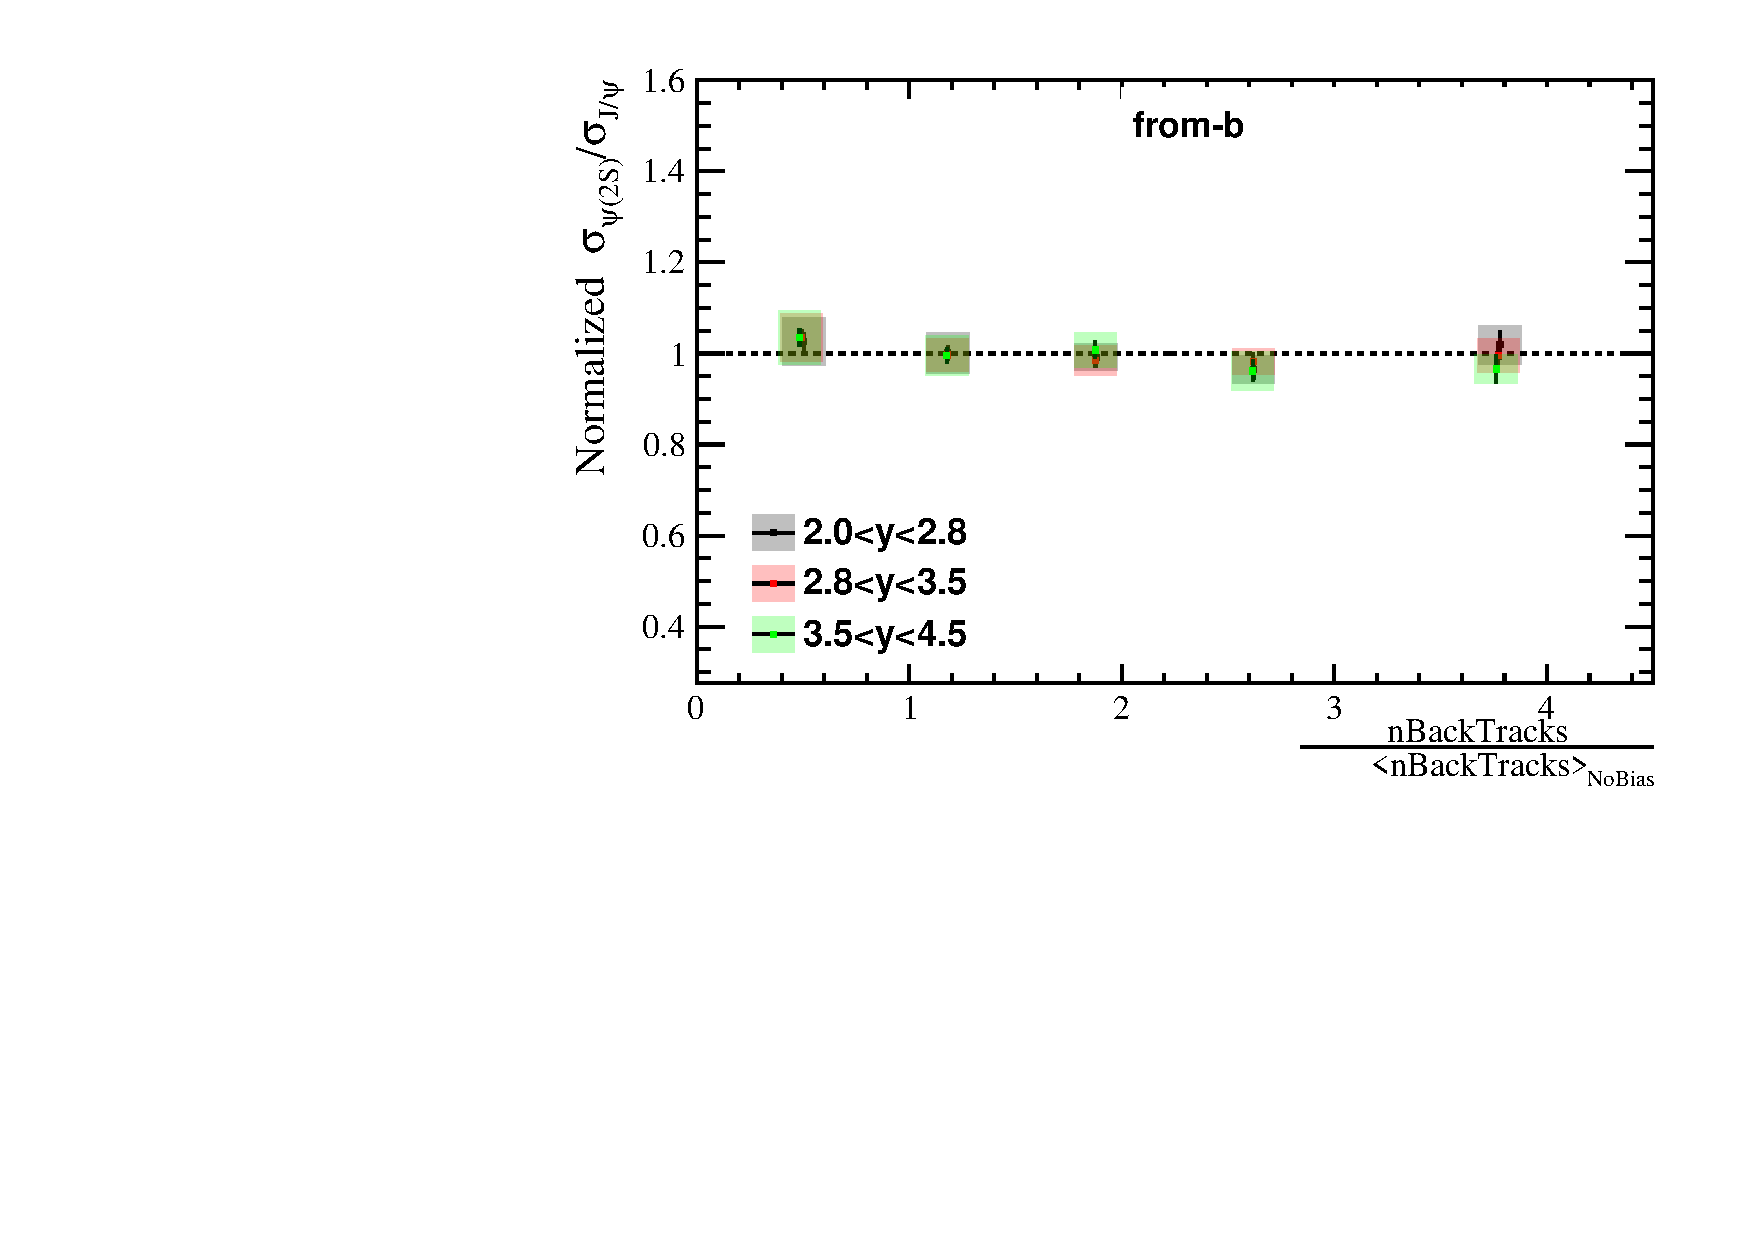
\includegraphics[width=0.48\linewidth]{pdf/Result/frombRatioYB.pdf}
  \end{center}
  \caption{Ratio of \psitwos to \jpsi in different $y$ region when multiplicity is divided in nBackTracks}.
  \label{RatioY_Back}
\end{figure}
\subsection{Comparisons with other measurements}
\label{Compare}
Measurements of $\BR_{\psitwos}/\sigma_{\psitwos}$ over $\BR_{\jpsi}/\sigma_{\jpsi}$ have been done in different collision systems at different center-of-mass energies. Results show that the value of the ratio is roughly independent of the collision systems and energies. We multiply the ratio of $\sigma_{\psitwos}/\sigma_{\jpsi}$ by the ratio of their branching fractions and add our measurements to the plot as follows, we find our measurements having a good agreement with others in Figs~\ref{compare_total} and Figs~\ref{compare_pt}.
\begin{figure}[H]
  \begin{center}
  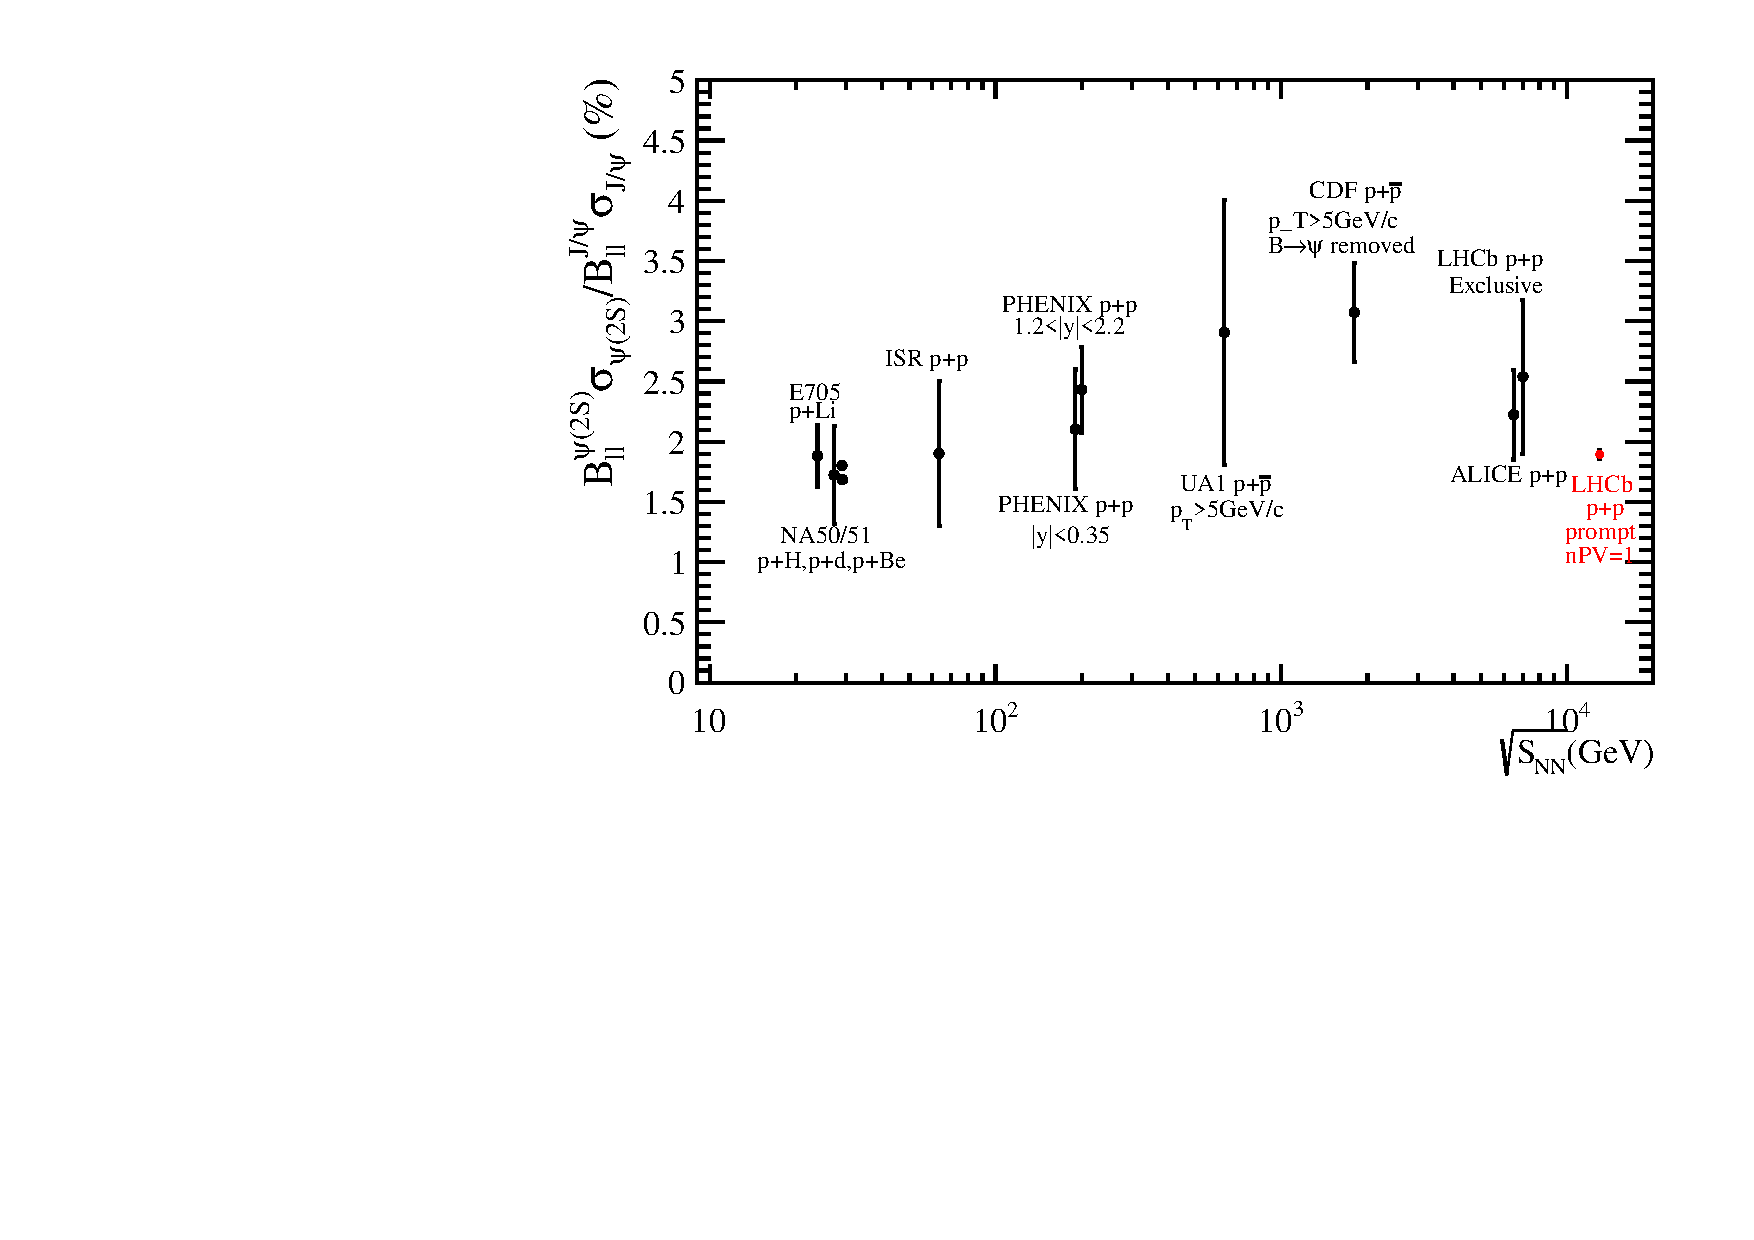
\includegraphics[width=0.7\linewidth]{pdf/Result/VariousMeasurements.pdf }
  \end{center}
  \caption{Comparisons of world data on the ratio of \psitwos/\jpsi measons in dilepton decays~\cite{PHENIX:2016vmz,NA50:2006rdp,PHENIX:2011gyb,E705:1992vec,NA51:1998uun,Clark:1978mg,UA1:1990eni,CDF:1997ykw,LHCb:2013nqs}.}
\label{compare_total}
\end{figure}
\begin{figure}[H]
  \begin{center}
  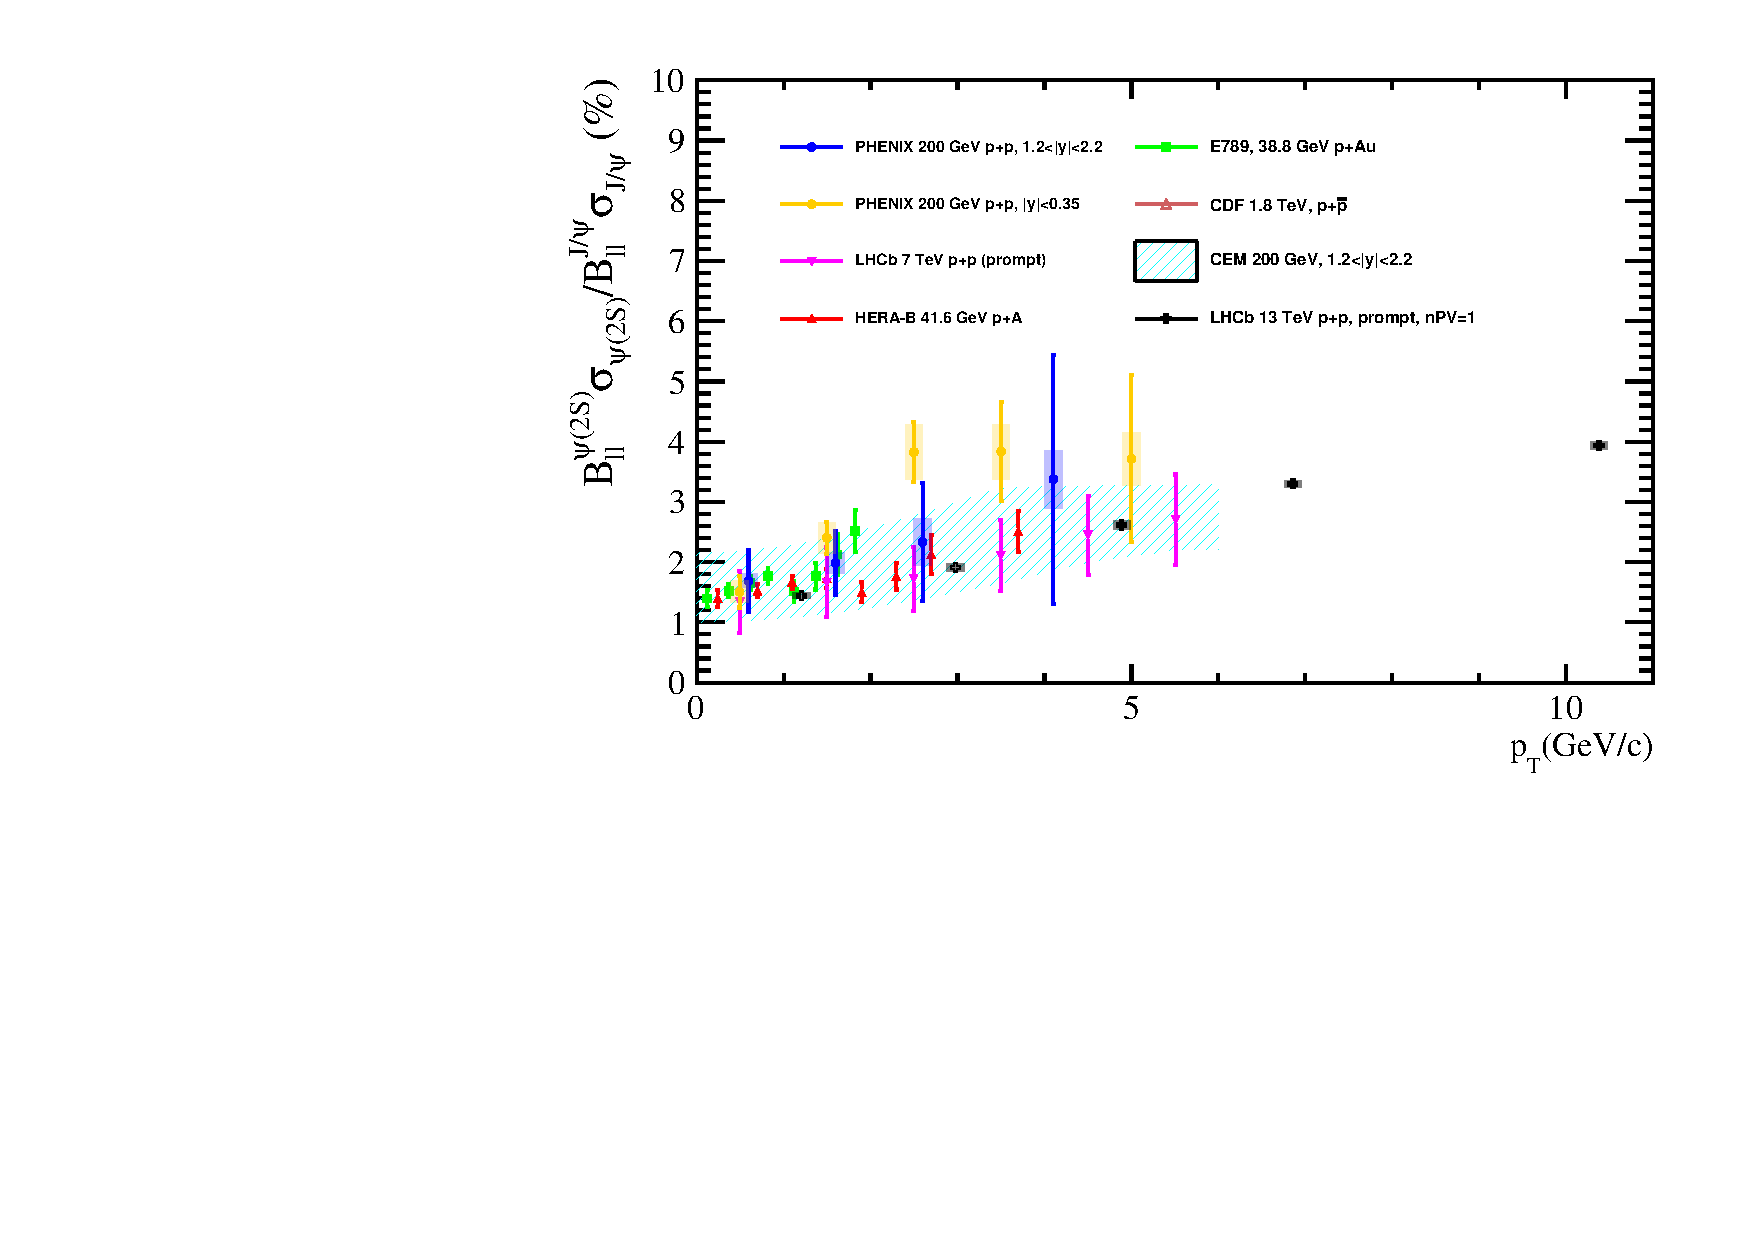
\includegraphics[width=0.7\linewidth]{pdf/Result/Comparisons_PT_VariousMeasurements.pdf}
  \end{center}
  \caption{Comparisons of world data on the ratio of \psitwos/\jpsi measons as a function of \pt in dilepton decays~\cite{PHENIX:2016vmz,NA50:2006rdp,PHENIX:2011gyb,E705:1992vec,NA51:1998uun,Clark:1978mg,UA1:1990eni,CDF:1997ykw,LHCb:2013nqs}.}
\label{compare_pt}
\end{figure}
